\chapter{Suites et séries de fonctions}

\minitoc

Dans ce chapitre, \(\K\) désigne \(\R\) ou \(\C\). Toutes les fonctions considérées vont de \(\R\) dans \(\K\) dans un premier temps. Dans un second temps, on généralisera les définitions et résultats à des fonctions de \(E\) dans \(F\), deux espaces vectoriels normés de dimension finies.

\section{Convergence d'une suite de fonctions}

Comme son nom l'indique, une suite de fonctions est une suite \(\paren{f_n}\) où \(f_n\) est une fonction de \(\R\) dans \(\K\).

\subsection{Convergence simple}

\begin{defi}
Soient \(A\) une partie de \(\R\) et \(\paren{f_n}\) une suite de fonctions définies sur \(A\).

On dit que la suite \(\paren{f_n}\) converge simplement sur \(A\) quand pour tout \(x\in A\), la suite numérique \(\paren{f_n\paren{x}}\) converge.

Dans ce cas, on peut définir une fonction \(f\) sur \(A\) en posant \(\quantifs{\tpt x\in A}f\paren{x}=\lim_{n\to\pinf}f_n\paren{x}\).

La fonction \(f\) est alors appelée limite simple sur \(A\) de la suite \(\paren{f_n}\) et on dit que la suite \(\paren{f_n}\) converge simplement vers \(f\) sur \(A\).
\end{defi}

On observe la définition formelle de la convergence simple sur \(A\) : \[\quantifs{\forall x\in A;\forall\epsilon>0;\exists n_0\in\N;\forall n\geq n_0}\abs{f_n\paren{x}-f\paren{x}}\leq\epsilon.\]

Le rang \(n_0\) dépend à la fois de \(x\) et de \(\epsilon\).

\begin{exo}
Étudiez la convergence simple de la suite de fonctions \(f_n:x\mapsto\dfrac{n\e{-x}+x^2}{n+x}\), où \(n>0\), sur \(\intervie{0}{\pinf}\).
\end{exo}

\begin{exo}
Même question avec la suite de fonctions \(f_n:x\mapsto\dfrac{x^n}{1+x^n}\), où \(n>0\), sur \(\intervie{0}{\pinf}\).
\end{exo}

\begin{exo}
Même question avec la suite de fonctions \(f_n:x\mapsto n^\alpha x^n\paren{1-x}\), où \(n>0\) et \(\alpha\in\Rps\), sur \(\intervii{0}{1}\). 
\end{exo}

\subsection{Convergence uniforme}

\begin{rappel}
Si \(g\) est une fonction bornée sur une partie \(A\) de \(\R\), on pose \(\norme{g}_\infty^A=\sup_{x\in A}\abs{g\paren{x}}\).

\(\norme{}_\infty^A\) est une norme sur le \(\K\)-espace vectoriel des fonctions bornées sur \(A\), appelée norme infinie ou norme uniforme sur \(A\).
\end{rappel}

Un résultat essentiel : la majoration de la norme uniforme.

\begin{prop}
Soient \(f\) une fonction bornée sur une partie \(A\) de \(\R\) et \(K\) un réel positif.

On a \[\norme{f}_\infty^A\leq K\ssi\quantifs{\forall x\in A}\abs{f\paren{x}}\leq K.\]
\end{prop}

\begin{defi}
Soient \(A\) une partie de \(\R\), \(\paren{f_n}\) une suite de fonctions définies sur \(A\) et \(f\) une fonction définie sur \(A\).

On dit que la suite \(\paren{f_n}\) converge uniformément vers \(f\) sur \(A\) quand pour tout \(n\in\N\), la fonction \(f-f_n\) est bornée sur \(A\) et la suite réelle \(\paren{\norme{f-f_n}_\infty^A}\) converge vers \(0\).

La fonction \(f\) est alors appelée limite uniforme sur \(A\) de la suite \(\paren{f_n}\).
\end{defi}

On observe la définition formelle de la convergence uniforme sur \(A\) : \[\quantifs{\forall\epsilon>0;\exists n_0\in\N;\forall n\geq n_0;\forall x\in A}\abs{f_n\paren{x}-f\paren{x}}\leq\epsilon.\]

Le rang \(n_0\) dépend seulement de \(\epsilon\) mais plus de \(x\) : c'est le même \(n_0\) pour toutes les valeurs de \(x\), en ce sens, il est uniforme.

Souvent, on ne sait pas calculer les normes uniformes des fonctions \(f_n-f\). Une simple majoration suffit, qu'on appelle majoration uniforme.

\begin{defi}
Soient \(A\) une partie de \(\R\) et \(\paren{f_n}\) une suite de fonctions définies sur \(A\).

On appelle majoration uniforme sur \(A\) toute proposition du type \[\quantifs{\forall n\in\N;\forall x\in A}\abs{f_n\paren{x}}\leq K_n\] où \(K_n\) est une constante indépendante de \(x\).
\end{defi}

\begin{ex}
\begin{itemize}
    \item La proposition \[\quantifs{\forall n\in\Ns;\forall x\in\R}\abs{\dfrac{\sin\paren{nx}}{n}}\leq\dfrac{1}{n}\] est une majoration uniforme des fonctions \(x\mapsto\dfrac{\sin\paren{nx}}{n}\) sur \(\R\). \\
    \item La proposition \[\quantifs{\forall n\in\Ns;\forall x\in\R}\abs{\dfrac{\sin\paren{nx}}{n+x^2}}\leq\dfrac{1}{n+x^2}\] n'est pas une majoration uniforme des fonctions \(x\mapsto\dfrac{\sin\paren{nx}}{n+x^2}\) sur \(\R\) car le majorant dépend de \(x\).
\end{itemize}
\end{ex}

\begin{exo}
Donnez une majoration uniforme des fonctions \(x\mapsto\dfrac{\ln\paren{1+nx}}{x}\) sur \(\intervee{0}{\pinf}\).
\end{exo}

\begin{corr}
On a \[\quantifs{\forall n\in\N;\forall x\in\intervee{0}{\pinf}}0\leq\dfrac{\ln\paren{1+nx}}{x}\leq\dfrac{nx}{x}=n.\]
\end{corr}

\begin{exo}
Même exercice avec les fonctions \(x\mapsto\dfrac{\sin\paren{nx}}{\sin x}\) sur \(\intervee{-\pi}{\pi}\excluant\accol{0}\).
\end{exo}

\begin{corr}
Pour \(n\in\N\), on pose \(\fonction{f_n}{\intervee{-\pi}{\pi}\excluant\accol{0}}{\R}{x}{\dfrac{\sin\paren{nx}}{\sin x}}\)

Soit \(n\in\N\).

Pour \(x\in\intervie{\dfrac{\pi}{6}}{\dfrac{5\pi}{6}}\), on a \(\dfrac{1}{2}\leq\sin x\) donc \[\abs{f_n}=\dfrac{\abs{\sin\paren{nx}}}{\sin x}\leq2\abs{\sin x}\leq2.\]

Pour \(x\in\intervei{0}{\dfrac{\pi}{6}}\), comme \(\sin\) est concave sur \(\intervei{0}{\dfrac{\pi}{6}}\), on a \(\dfrac{3}{\pi}x\leq\sin x\) et donc \[\abs{f_n\paren{x}}=\dfrac{\abs{\sin\paren{nx}}}{\sin x}\leq\dfrac{\abs{\sin\paren{nx}}}{x}\times\dfrac{\pi}{3}\leq\dfrac{\abs{nx}}{x}\times\dfrac{\pi}{3}=\dfrac{n\pi}{3}.\]

Pour \(x\in\intervie{\dfrac{5\pi}{6}}{\pi}\), on pose \(t=\pi-x\in\intervei{0}{\dfrac{\pi}{6}}\) et on a \[\dfrac{\sin\paren{nx}}{\sin x}=\dfrac{\sin\paren{n\paren{\pi-t}}}{\sin\paren{\pi-t}}=\dfrac{\paren{-1}^n\sin\paren{-nt}}{\sin t}=\dfrac{\paren{-1}^{n+1}\sin\paren{nt}}{\sin t}\] donc \[\abs{f_n\paren{x}}=\abs{\dfrac{\sin\paren{nt}}{\sin t}}\leq\dfrac{n\pi}{3}.\]

Finalement, \(\quantifs{\tpt x\in\intervee{0}{\pi}}\abs{f_n\paren{x}}\leq\max\paren{2,\dfrac{n\pi}{3}}\).

De plus, \(\abs{f_n}\) est paire donc ceci reste vrai sur \(\intervee{-\pi}{0}\).
\end{corr}

\begin{prop}
Avec les mêmes hypothèses, il y a équivalence entre

\begin{enumerate}
    \item la suite \(\paren{f_n}\) converge uniformément vers \(f\) sur \(A\) \\
    \item il existe une suite positive \(\paren{\alpha_n}\) telle que \(\quantifs{\tpt n\in\N}\norme{f_n-f}_\infty^A\leq\alpha_n\) et \(\alpha_n\tendqd{n\to\pinf}0\) \\
    \item il existe une majoration uniforme des fonctions \(f_n-f\) sur \(A\) par les termes d'une suite numérique positive qui converge vers \(0\), \ie on a une proposition du type \[\quantifs{\forall n\in\N;\forall x\in A}\abs{f_n\paren{x}-f\paren{x}}\leq\alpha_n\qquad\text{et}\qquad\alpha_n\tendqd{n\to\pinf}0\] où \(\alpha_n\) ne dépend pas de \(x\).
\end{enumerate}
\end{prop}

\begin{dem}
(1) \(\imp\) (2) : on prend \(\alpha_n=\norme{f_n-f}_\infty^A\).

(2) \(\imp\) (1) : théorème d'encadrement.

(2) \(\ssi\) (3) : \(\norme{f_n-f}_\infty^A\leq\alpha_n\ssi\quantifs{\forall x\in A}\abs{f_n\paren{x}-f\paren{x}}\leq\alpha_n\).
\end{dem}

Il y a un lien entre convergence simple et uniforme, dans un seul sens !

\begin{theo}
Si une suite \(\paren{f_n}\) converge uniformément vers \(f\) sur \(A\), alors \(\paren{f_n}\) converge simplement vers \(f\) sur \(A\).
\end{theo}

\begin{dem}
On a \(\quantifs{\forall x\in A}\abs{f_n\paren{x}-f\paren{x}}\leq\norme{f_n-f}_\infty^A\).

Donc si \(\paren{f_n}\) converge uniformément vers \(f\) sur \(A\), \(\norme{f_n-f}_\infty^A\tendqd{n\to\pinf}0\).

Donc \(\abs{f_n\paren{x}-f\paren{x}}\tendqd{n\to\pinf}0\) par encadrement, \ie \(f_n\paren{x}\tendqd{n\to\pinf}f\paren{x}\) \ie \(\paren{f_n}\) converge simplement vers \(f\) sur \(A\).
\end{dem}

La réciproque est fausse ! Contre-exemple : la suite de fonctions \(\paren{x\mapsto x^n}\) sur \(\intervii{0}{1}\).

\begin{dem}
On pose \(f_n:x\mapsto x^n\) sur \(\intervii{0}{1}\).

\(\paren{f_n}\) converge simplement vers \(f:x\mapsto\begin{dcases}
0 &\text{si }x\in\intervie{0}{1} \\
1 &\text{sinon}
\end{dcases}\)

On a \[\norme{f_n-f}_\infty^{\intervii{0}{1}}=\sup_{x\in\intervii{0}{1}}\abs{x^n-f\paren{x}}=1\ntendqd{n\to\pinf}0.\]

Donc \(\paren{f_n}\) ne converge pas uniformément sur \(\intervii{0}{1}\).
\end{dem}

Conséquence : pour étudier la convergence uniforme d'une suite de fonctions, on commence par étudier sa convergence simple, car d'abord on détermine sa limite simple \(f\), puis on cherche à savoir si elle est limite uniforme.

\begin{exo}
Étudiez la convergence uniforme de la suite de fonctions \(f_n:x\mapsto\dfrac{n\e{-x}+x^2}{n+x}\), où \(n>0\), sur \(\intervii{0}{1}\).
\end{exo}

\begin{corr}
\(\quantifs{\Tpt x\in\intervii{0}{1}}f_n\paren{x}=\dfrac{n\e{-x}+x^2}{n+x}\tendqd{n\to\pinf}\e{-x}\) donc \(\paren{f_n}\) converge simplement vers \(f:x\mapsto\e{-x}\) sur \(\intervii{0}{1}\).

Pour \(n\in\Ns\) et \(x\in\intervii{0}{1}\), on a \[\begin{aligned}
\abs{f_n\paren{x}-f\paren{x}}&=\abs{\dfrac{n\e{-x}+x^2}{n+x}-\e{-x}} \\
&=\abs{\dfrac{x^2-x\e{-x}}{n+x}} \\
&\leq\dfrac{\abs{x^2}+\abs{x\e{-x}}}{n+x} \\
&=\dfrac{2}{n}.
\end{aligned}\]

Donc \(\norme{f_n-f}_\infty^{\intervii{0}{1}}\leq\dfrac{2}{n}\) et, par encadrement, on a \[\norme{f_n-f}_\infty^{\intervii{0}{1}}\tendqd{n\to\pinf}0\] \ie \(\paren{f_n}\) converge uniformément vers \(f\) sur \(\intervii{0}{1}\).

De même, on peut montrer la convergence uniforme sur \(\intervii{0}{b}\) pour tout \(b>0\).

En revanche, il n'y a pas convergence uniforme sur \(\intervie{0}{\pinf}\) car \(\lim_{x\to\pinf}\abs{f_n\paren{x}-f\paren{x}}=\pinf\) donc \(f_n-f\) n'est pas bornée sur \(\intervie{0}{\pinf}\) donc \(\norme{f_n-f}_\infty^{\intervie{0}{\pinf}}\) n'est pas défini.
\end{corr}

\begin{rem}
Cet exemple prouve que la convergence uniforme n'est pas préservée par réunion d'intervalles.
\end{rem}

\begin{exo}
Même question avec la suite de fonctions \(f_n:x\mapsto\dfrac{x^n}{1+x^n}\), où \(n>0\), sur \(\intervie{0}{\pinf}\).
\end{exo}

\begin{corr}
\(\paren{f_n}\) converge simplement vers \(f:x\mapsto\begin{dcases}
0 &\text{si }x<1 \\
\nicefrac{1}{2} &\text{si }x=1 \\
1 &\text{sinon}
\end{dcases}\) sur \(\intervie{0}{\pinf}\).

On a \(f_n-f:x\mapsto\begin{dcases}
\dfrac{x^n}{1+x^n} &\text{si }x<1 \\
0 &\text{si }x=1 \\
\dfrac{-1}{1+x^n} &\text{sinon}
\end{dcases}\) donc \(\abs{f_n-f}:x\mapsto\begin{dcases}
\dfrac{x^n}{1+x^n} &\text{si }x<1 \\
0 &\text{si }x=1 \\
\dfrac{1}{1+x^n} &\text{sinon}
\end{dcases}\)

On remarque \(\lim_{x\to1^+}\abs{f_n\paren{x}-f\paren{x}}=\dfrac{1}{2}\) donc \(\norme{f_n-f}_\infty^{\intervie{0}{\pinf}}\geq\dfrac{1}{2}\).

Donc \(\paren{f_n}\) ne converge pas uniformément sur \(\intervie{0}{\pinf}\).
\end{corr}

\begin{exo}
Même question avec la suite de fonctions \(f_n:x\mapsto n^\alpha x^n\paren{1-x}\), où \(n>0\) et \(\alpha\in\Rps\), sur \(\intervii{0}{1}\).
\end{exo}

\begin{corr}~\\
Si \(x<1\), alors \(\dfrac{1}{x}>1\) et donc \(n^\alpha\egqd{n\to\pinf}\o{\dfrac{1}{x^n}}\), donc \(\lim_{n\to\pinf}n^\alpha x^n=0\) et enfin \[\lim_{n\to\pinf}f_n\paren{x}=0.\]

Si \(x=1\), on a \(f_n\paren{1}=0\tendqd{n\to\pinf}0\).

Donc \(\paren{f_n}\) converge simplement vers la fonction nulle sur \(\intervii{0}{1}\).

Comme \(f_n\) est continue sur le compact \(\intervii{0}{1}\), on a \[\norme{f_n}_\infty^{\intervii{0}{1}}=\sup_{\intervii{0}{1}}\abs{f_n}=\sup_{\intervii{0}{1}}f_n=\max_{\intervii{0}{1}}f_n.\]

De plus, pour \(x\in\intervii{0}{1}\), on a \[\begin{aligned}
f_n\prim\paren{x}&=n^\alpha\paren{nx^{n-1}-\paren{n+1}x^n} \\
&=n^\alpha x^{n-1}\paren{n-\paren{n+1}x}.
\end{aligned}\]

On a donc le tableau de variations suivant :

\begin{center}
\begin{tikzpicture}
\tableauinit{\(x\) / 1, \(f_n\prim\paren{x}\) / 1, \(f_n\) / 2}{\(0\), \(\dfrac{n}{n+1}\), \(1\)}
\tableausignes{z,+,z,-,}
\tableauvariations{-/\(0\), +/, -/\(0\)}
\end{tikzpicture}
\end{center}

Donc \[\norme{f_n}_\infty^{\intervii{0}{1}}=f_n\paren{\dfrac{n}{n+1}}=n^\alpha\paren{\dfrac{n}{n+1}}^n\paren{\dfrac{1}{n+1}}.\]

De plus, on a \(\paren{\dfrac{n}{n+1}}^n=\exp\paren{n\ln\dfrac{n}{n+1}}\).

Or \[n\ln\dfrac{n}{n+1}=n\ln\dfrac{1}{1+\nicefrac{1}{n}}=-n\ln\paren{1+\dfrac{1}{n}}\simqd{n\to\pinf}\dfrac{-n}{n}\tendqd{n\to\pinf}-1.\]

Donc \(\exp\paren{n\ln\dfrac{n}{n+1}}\tendqd{n\to\pinf}\e{-1}\).

Donc \(\norme{f_n}_\infty^{\intervii{0}{1}}\simqd{n\to\pinf}\dfrac{n^{\alpha-1}}{\e{}}\).

Donc \(\norme{f_n}_\infty^{\intervii{0}{1}}\tendqd{n\to\pinf}0\) ssi \(\alpha<1\).

Enfin, \(\paren{f_n}\) converge uniformément vers la fonction nulle sur \(\intervii{0}{1}\) ssi \(\alpha<1\).
\end{corr}

Pour montrer la non-convergence uniforme, on dispose d'un critère simple suffisant dans bien des cas.

\begin{prop}
Soit \(\paren{f_n}\) une suite de fonctions qui converge simplement vers \(f\) sur une partie \(A\) de \(\R\).

S'il existe une suite \(\paren{x_n}\) à termes dans \(A\) telle que la suite \(\paren{f\paren{x_n}-f_n\paren{x_n}}\) ne converge pas vers \(0\), alors la suite \(\paren{f_n}\) ne converge pas uniformément sur \(A\).
\end{prop}

\begin{dem}
On a \(\norme{f_n-f}_\infty^A\geq\abs{f\paren{x_n}-f_n\paren{x_n}}\), d'où la proposition.
\end{dem}

\begin{exo}
Montrez que la suite de fonctions \(f_n:x\mapsto x^2\cos\dfrac{x}{n}\) converge simplement sur \(\R\) vers une fonction \(f\) à préciser.

Montrez que la convergence n'est pas uniforme sur \(\R\), mais qu'elle l'est sur tout segment \(\intervii{0}{a}\).
\end{exo}

\begin{corr}
\(\paren{f_n}\) converge simplement vers \(f:x\mapsto x^2\) sur \(\R\).

On pose \(x_n=n\pi\) et on a \[f_n\paren{x_n}-f\paren{x_n}=\paren{n\pi}^2\cos\paren{\pi}-\paren{n\pi}^2=-2n^2\pi^2\tendqd{n\to\pinf}\minf.\]

Donc \(\paren{f_n\paren{x_n}-f\paren{x_n}}\) ne converge pas vers \(0\) et donc \(\paren{f_n}\) ne converge pas uniformément vers \(f\) sur \(\R\).

Soit \(a>0\). Pour \(x\in\intervii{0}{a}\), on a \[\begin{aligned}
\abs{x^2\cos\dfrac{x}{n}-x^2}&=\abs{x^2\paren{\cos\dfrac{x}{n}-1}} \\
&=\abs{x^2}\abs{\cos\dfrac{x}{n}-1} \\
&\leq a^2\abs{\cos\dfrac{x}{n}-1}.
\end{aligned}\]

Or \(\cos\paren{0}=1\) et \(\abs{\cos\prim}=\abs{-\sin}\leq1\) donc d'après l'inégalité des accroissements finis, on a \[\abs{\cos\dfrac{x}{n}-\cos\paren{0}}\leq1\abs{\dfrac{x}{n}-0}.\]

Donc \(\abs{\cos\dfrac{x}{n}-1}\leq\dfrac{x}{n}\leq\dfrac{a}{n}\) et donc \[\abs{x^2\cos\dfrac{x}{n}-x^2}\leq\dfrac{a^3}{n}.\]

Or \(\dfrac{a^3}{n}\tendqd{n\to\pinf}0\) donc \(\norme{f-f_n}_\infty^{\intervii{0}{a}}\tendqd{n\to\pinf}0\).

Donc \(\paren{f_n}\) converge uniformément vers \(f\) sur \(\intervii{0}{a}\).
\end{corr}

\section{Convergence d'une série de fonctions}

\subsection{Convergence simple}

\begin{defi}
Soient \(A\) une partie de \(\R\) et \(\paren{f_n}\) une suite de fonctions définies sur \(A\).

On dit que la série \(\sum_{n\geq0}f_n\) converge simplement sur \(A\) quand pour tout \(x\in A\), la série numérique \(\sum_{n\geq0}f_n\paren{x}\) converge.

Autrement dit, la série de fonctions \(\sum_{n\geq0}f_n\) converge simplement sur \(A\) quand la suite des sommes partielles \(\paren{\sum_{k=0}^nf_k}\) converge simplement sur \(A\).

Dans ce cas, on peut définir une fonction \(f\) sur \(A\) en posant \(\quantifs{\tpt x\in A}f\paren{x}=\sum_{n=0}^{\pinf}f_n\paren{x}\).

La fonction \(f\) est alors appelée (fonction) somme sur \(A\) de la série \(\sum_{n\geq0}f_n\).
\end{defi}

\begin{exo}
Étudiez la convergence simple de la série de fonctions \(f_n:x\mapsto\dfrac{nx^2}{n^3+x^2}\), où \(n\geq0\), sur \(\intervie{0}{\pinf}\).
\end{exo}

\begin{corr}\thlabel{corr11.10}
On a \(f_n\paren{x}\simqd{n\to\pinf}\dfrac{x^2}{n^2}\) donc par théorème de comparaison des séries à termes positifs, \(\sum_nf_n\paren{x}\) converge.

Donc \(\sum_nf_n\) converge simplement sur \(\intervie{0}{\pinf}\).
\end{corr}

\begin{exo}
Même question avec la série de fonctions \(f_n:x\mapsto\dfrac{x^n}{1+x^n}\), où \(n>0\), sur \(\intervie{0}{\pinf}\).
\end{exo}

\begin{corr}\thlabel{corr11.11}
Si \(x\in\intervie{0}{1}\), on a \(f_n\paren{x}\simqd{n\to\pinf}x^n\) donc par théorème de comparaison des séries à termes positifs, \(\sum_nf_n\paren{x}\) converge et donc \(\sum_nf_n\) converge simplement.

Si \(x=1\), \(\sum_nf_n\paren{x}=\sum_n\dfrac{1}{2}\) diverge grossièrement.

Si \(x\in\intervie{1}{\pinf}\), \(f_n\paren{x}\tendqd{n\to\pinf}1\) donc \(\sum_nf_n\paren{x}\) diverge grossièrement.
\end{corr}

\begin{exo}
Même question avec la série de fonctions \(f_n:x\mapsto\dfrac{\sin\paren{nx}}{n^3+x^3}\), où \(n>0\), sur \(\intervie{0}{\pinf}\).
\end{exo}

\begin{corr}
On a \[\abs{f_n\paren{x}}=\dfrac{\abs{\sin\paren{nx}}}{n^3+x^3}\leq\dfrac{1}{n^3}\] donc par théorème de comparaison des séries à termes positifs, \(\sum_nf_n\paren{x}\) converge absolument et donc converge, donc \(\sum_nf_n\) converge simplement.
\end{corr}

\subsection{Convergence uniforme}

On a la même définition en remplaçant \guillemets{simple} par \guillemets{uniforme}.

\begin{defi}
Soient \(A\) une partie de \(\R\) et \(\paren{f_n}\) une suite de fonctions définies sur \(A\).

On dit que la série \(\sum_{n\geq0}f_n\) converge uniformément sur \(A\) quand la suite des sommes partielles \(\paren{\sum_{k=0}^nf_k}\) converge uniformément sur \(A\).

La fonction somme \(f\) est alors appelée limite uniforme sur \(A\) de la série \(\sum_{n\geq0}f_n\).
\end{defi}

Encore une fois, il y a un lien entre la convergence simple et uniforme, dans un seul sens !

\begin{theo}
Si une série de fonctions \(\sum_{n\geq0}f_n\) converge uniformément sur \(A\), alors \(\sum_{n\geq0}f_n\) converge simplement sur \(A\).
\end{theo}

La réciproque est fausse ! Contre-exemple : la série de fonctions \(\sum_{n\geq0}\paren{x\mapsto x^n}\).

\begin{dem}~\\
On a \(\sum_{k=0}^nf_k\paren{x}=\dfrac{1-x^{n+1}}{1-x}\) et \(\sum_{n=0}^{\pinf}f_n\paren{x}=\dfrac{1}{1-x}=f\paren{x}\) donc \[\begin{aligned}
\sum_{k=0}^n f_k\paren{x}-f\paren{x}&=\dfrac{-x^{n+1}}{1-x} \\
\abs{\sum_{k=0}^nf_k\paren{x}-f\paren{x}}&=\dfrac{x^{n+1}}{1-x} \\
&\tendqd{x\to1^-}\pinf.
\end{aligned}\]

Donc \(\sum_{k=0}^nf_k-f\) n'est pas bornée sur \(\intervie{0}{1}\).
\end{dem}

On peut réécrire la définition à l'aide des restes partiels.

\begin{prop}
Soit \(A\) une partie de \(\R\).

La série \(\sum_{n\geq0}f_n\) converge uniformément sur \(A\) quand la série \(\sum_{n\geq0}f_n\) converge simplement sur \(A\) et la suite des restes partiels \(\paren{\sum_{k=n+1}^{\pinf}f_k}\) converge uniformément vers \(0\) sur \(A\), \ie \(\norme{\sum_{k=n+1}^{\pinf}f_k}_\infty^A\tendqd{n\to\pinf}0\).
\end{prop}

Il suffit donc qu'il existe une suite positive \(\paren{\alpha_n}\) telle que \(\norme{\sum_{k=n+1}^{\pinf}f_k}_\infty^A\leq\alpha_n\) et \(\alpha_n\tendqd{n\to\pinf}0\) pour que la série \(\sum_{n\geq0}f_n\) converge uniformément vers \(f\) sur \(A\).

Autrement dit, il suffit de trouver une majoration uniforme des restes partiels par les termes d'une suite positive qui converge vers \(0\).

\begin{exo}
Étudiez la convergence uniforme de la série de fonctions \(f_n:x\mapsto\dfrac{\paren{-1}^n}{x+n}\), où \(n>0\), sur \(\intervie{0}{\pinf}\).
\end{exo}

\begin{corr}
Pour \(x\in\intervie{0}{\pinf}\), la suite \(\paren{\dfrac{1}{x+n}}_{n\geq1}\) est positive, décroissante et converge vers \(0\) donc d'après le critère spécial des séries alternées, \(\sum_nf_n\paren{x}\) converge et donc \(\sum_nf_n\) converge simplement.

Pour \(n\geq1\), on a \[\abs{\sum_{k=0}^{\pinf}f_k\paren{x}-\sum_{k=0}^nf_k\paren{x}}=\abs{\sum_{k=n+1}^{\pinf}f_k\paren{x}}\leq\dfrac{1}{x+n+1}\leq\dfrac{1}{n+1}.\]

(Majoration uniforme par une suite convergeant vers \(x\)).
\end{corr}

\begin{exo}
Même question avec la série de fonctions \(f_n:x\mapsto\dfrac{\paren{-1}^n\e{-nx}}{n}\), où \(n>0\), sur \(\intervie{0}{\pinf}\).
\end{exo}

\begin{corr}
Idem, pour \(x\in\intervie{0}{\pinf}\), la suite \(\paren{\dfrac{\e{-nx}}{n}}\) est positive, décroissante et converge vers \(0\) donc d'après le critère spéciale des séries alternées, \(\sum_nf_n\paren{x}\) converge.

De plus, on a \[\abs{\sum_{k=n+1}^{\pinf}\dfrac{\paren{-1}^k\e{-kx}}{k}}\leq\dfrac{\e{-\paren{n+1}x}}{n+1}\leq\dfrac{1}{n+1}.\]
\end{corr}

De manière analogue aux séries numériques, on note le lien entre la convergence uniforme d'une série de fonctions \(\sum_{n\geq0}u_n\) et la convergence uniforme de la suite \(\paren{u_n}\).

\begin{prop}
Soient \(A\) une partie de \(\R\) et \(\paren{u_n}\) une suite de fonctions définies sur \(A\).

Si la série \(\sum_{n\geq0}u_n\) converge uniformément sur \(A\), alors la suite \(\paren{u_n}\) converge uniformément vers \(0\).
\end{prop}

\begin{dem}~\\
On a \(u_n=\sum_{k=n}^{\pinf}f_k-\sum_{k=n+1}^{\pinf}f_k\) donc \[\norme{u_n}_\infty^A\leq\norme{\sum_{k=n}^{\pinf}f_k}_\infty^A+\norme{\sum_{k=n+1}^{\pinf}f_k}_\infty^A.\]

Donc si \(\sum_nf_n\) converge uniformément sur \(A\), alors \[\norme{\sum_{k=n}^{\pinf}f_k}_\infty^A\tendqd{n\to\pinf}0.\]

Donc, par encadrement, \(\norme{u_n}_\infty^A\tendqd{n\to\pinf}0\) \ie \(\paren{u_n}\) converge uniformément vers \(0\).
\end{dem}

Évidemment, la réciproque est fausse.

\subsection{Convergence normale}

Ce dernier type de convergence est spécifique aux séries de fonctions.

\begin{defi}
Soient \(A\) une partie de \(\R\) et \(\paren{f_n}\) une suite de fonctions définies sur \(A\).

On dit que la série \(\sum_{n\geq0}f_n\) converge normalement sur \(A\) quand la série numérique \(\sum_{n\geq0}\norme{f}_\infty^A\) converge.
\end{defi}

Souvent, on ne sait pas calculer les normes uniformes des fonctions \(f_n\). Une simple majoration suffit.

\begin{prop}
Avec les mêmes hypothèses, il y a équivalence entre

\begin{itemize}
    \item la série \(\sum_{n\geq0}f_n\) converge normalement sur \(A\) \\
    \item il existe une suite positive \(\paren{\alpha_n}\) telle que \(\quantifs{\tpt n\in\N}\norme{f_n}_\infty^A\leq\alpha_n\) et la série \(\sum_{n\geq0}\alpha_n\) converge \\
    \item il existe une majoration uniforme des fonctions \(f_n\) sur \(A\) par les termes d'une série positive convergente.
\end{itemize}
\end{prop}

Il y a un lien entre convergence uniforme et normale, dans un seul sens !

\begin{theo}
Si une série de fonctions converge normalement sur \(A\), alors elle converge uniformément sur \(A\). Elle converge aussi absolument sur \(A\).
\end{theo}

\begin{dem}
Si \(\sum_nf_n\) converge normalement sur \(A\), alors \[\quantifs{\forall n\in\N;\forall x\in A}\abs{f_n\paren{x}}\leq\norme{f_n}_\infty^A.\]

Or \(\norme{f_n}_\infty^A\) est le terme général d'une série convergente donc \(\sum_nf_n\paren{x}\) converge absolument.

Donc \(\sum_nf_n\) converge simplement sur \(A\).

De plus, \[\begin{WithArrows}
\norme{\sum_{k=n+1}^{\pinf}f_k}_\infty^A&\leq\sum_{k=n+1}^{\pinf}\norme{f_k}_\infty^A \Arrow{reste partiel d'une série convergente} \\
&\tendqd{n\to\pinf}0.
\end{WithArrows}\]

Donc, par encadrement, \(\norme{\sum_{k=n+1}^{\pinf}f_k}_\infty^A\tendqd{n\to\pinf}0\) \ie \(\sum_nf_n\) converge uniformément sur \(A\).
\end{dem}

La réciproque est fausse ! Contre-exemple : la série de fonctions \(\sum_{n\geq2}\paren{x\mapsto\dfrac{x^n}{\ln n}-\dfrac{x^{n+1}}{\ln\paren{n+1}}}\) converge uniformément sur \(\intervii{0}{1}\) mais pas normalement.

En pratique, il est souvent plus simple de montrer la convergence normale que la convergence uniforme d'une série. On commence donc par étudier la convergence simple, puis la convergence normale et, en cas d'échec, la convergence uniforme.

\begin{exo}
Étudiez la convergence uniforme de la série de fonctions \(f_n:x\mapsto\dfrac{nx^2}{n^3+x^2}\), où \(n>0\), sur \(\intervie{0}{\pinf}\).
\end{exo}

\begin{corr}
D'après la \thref{corr11.10}, \(\sum_nf_n\) converge simplement sur \(\intervie{0}{\pinf}\).

\(\sum_n\norme{f_n}_\infty^{\intervie{0}{\pinf}}\) converge-t-elle ?

Pour \(n\geq1\) et \(x\in\intervie{0}{\pinf}\), on a \[f_n\prim\paren{x}=\dfrac{2nx\paren{n^3+x^2}-nx^2\paren{2x}}{\paren{n^3+x^2}^2}=\dfrac{2n^4x}{\paren{n^3+x^2}^2}.\]

Donc on a le tableau de variations suivant :

\begin{center}
\begin{tikzpicture}
\tableauinit{\(x\) / 1, \(f_n\prim\paren{x}\) / 1, \(f_n\) / 2}{\(0\), \(\pinf\)}
\tableausignes{z,+,}
\tableauvariations{-/\(0\), +/\(n\)}
\end{tikzpicture}
\end{center}

Donc \(\norme{f_n}_\infty^{\intervie{0}{\pinf}}\geq n\) et donc on n'a pas convergence normale sur \(\intervie{0}{\pinf}\).

Soit \(a>0\). \(\sum_n\norme{f_n}_\infty^{\intervii{0}{a}}\) converge-t-elle ?

Pour \(n\in\Ns\), \(f_n\) est croissante sur \(\intervii{0}{a}\) donc \[\norme{f_n}_\infty^{\intervii{0}{a}}=f_n\paren{a}=\dfrac{na^2}{n^3+a^2}\] donc \(\sum_nf_n\) converge normalement sur \(\intervii{0}{a}\) et donc converge uniformément sur \(\intervii{0}{a}\).

En posant \(R_n\paren{x}=\sum_{k=n+1}^{\pinf}\dfrac{kx^2}{k^3+x^2}\) et \(S_n\paren{x}=\sum_{k=n+1}^{2n}\dfrac{kx^2}{k^3+x^2}\), on a \[R_n\paren{x}\geq S_n\paren{x}.\]

De plus, on a \[\begin{aligned}
\lim_{x\to\pinf}\sum_{k=n+1}^{2n}\dfrac{kx^2}{k^3+x^2}&=\sum_{k=n+1}^{2n}\lim_{x\to\pinf}\dfrac{kx^2}{k^3+x^2} \\
&=\sum_{k=n+1}^{2n}k \\
&\geq n^2.
\end{aligned}\]

On veut montrer \(\norme{R_n}_\infty^{\intervie{0}{\pinf}}\ntendqd{n\to\pinf}0\).

On a \(R_n\paren{x}\geq S_n\paren{x}\) et \(\lim_{x\to\pinf}S_n\paren{x}\geq n^2\) donc il existe \(a_n>0\) tel que \[\quantifs{\forall x\in\intervie{a_n}{\pinf}}S_n\paren{x}\geq\dfrac{n^2}{2}\] donc \[\quantifs{\forall x\in\intervie{a_n}{\pinf}}R_n\paren{x}\geq\dfrac{n^2}{2}\] donc \[\norme{R_n}_\infty^{\intervie{0}{\pinf}}\geq\dfrac{n^2}{2}.\]

Donc la convergence n'est pas uniforme sur \(\intervie{0}{\pinf}\).
\end{corr}

\begin{exo}
Même question avec la série de fonctions \(f_n:x\mapsto\dfrac{x^n}{1+x^n}\), où \(n>0\), sur \(\intervie{0}{\pinf}\).
\end{exo}

\begin{corr}
D'après la \thref{corr11.11}, \(\sum_nf_n\) converge simplement sur \(\intervie{0}{1}\).

On étudie d'abord la convergence normale de la série \(\sum_nf_n\).

Pour \(n\in\Ns\), on a \[\begin{aligned}
\odv*{\dfrac{x^n}{x^n+1}}{x}&=\dfrac{nx^{n-1}\paren{1+x^n}-x^n\paren{nx^{n-1}}}{\paren{1+x^n}^2} \\
&=\dfrac{nx^{n-1}+nx^{2n-1}-nx^{2n-1}}{\paren{1+x^n}^2} \\
&=\dfrac{nx^{n-1}}{\paren{1+x^n}^2}.
\end{aligned}\]

On a donc le tableau de variations suivant :

\begin{center}
\begin{tikzpicture}
\tableauinit{\(x\) / 1, \(f_n\) / 2}{\(0\), \(1\)}
\tableauvariations{-/\(0\), +/\(\nicefrac{1}{2}\)}
\end{tikzpicture}
\end{center}

Donc \(\norme{f_n}_\infty^{\intervie{0}{1}}=\dfrac{1}{2}\).

Donc \(\sum_n\norme{f_n}_\infty^{\intervie{0}{1}}\) diverge grossièrement.

Donc \(\sum_nf_n\) ne converge pas normalement.

Pour \(a\in\intervie{0}{1}\), \(\norme{f_n}_\infty^{\intervii{0}{a}}=f_n\paren{a}\) et \(\sum_nf_n\paren{a}\) converge donc \(\sum_nf_n\) converge normalement sur \(\intervii{0}{a}\) et donc uniformément sur \(\intervii{0}{a}\).
\end{corr}

\begin{exo}
Même question avec la série de fonctions \(f_n:x\mapsto\dfrac{x^2}{1+n^3x^3}\), où \(n>0\), sur \(\intervie{0}{\pinf}\).
\end{exo}

\begin{corr}
Si \(x=0\), \(f_n\paren{0}=0\) donc \(\sum_nf_n\paren{0}\) converge.

Si \(x>0\), \(f_n\paren{x}\simqd{n\to\pinf}\dfrac{1}{n^3x}\) donc par théorème de comparaison des séries à termes positifs, \(\sum_nf_n\paren{x}\) converge.

Donc \(\sum_nf_n\) converge simplement sur \(\intervie{0}{\pinf}\).

Pour \(x>0\), \(\abs{f_n\paren{x}}=f_n\paren{x}\leq\dfrac{1}{n^3x}\).

Si \(a>0\), pour tout \(x\in\intervie{a}{\pinf}\), on a \(\abs{f_n\paren{x}}\leq\dfrac{1}{an^3}\) donc \[\norme{f_n}_\infty^{\intervie{a}{\pinf}}\leq\dfrac{1}{an^3}\] donc \(\sum_nf_n\) converge normalement et donc uniformément sur \(\intervie{a}{\pinf}\).

Pour tout \(x\geq0\), on a \(1\leq1+n^3x^3\) donc \(\dfrac{1}{1+n^3x^3}\leq1\) donc \(f_n\paren{x}\leq x^2\).

Donc \(\quantifs{\tpt x\in\intervii{0}{\dfrac{1}{n}}}0\leq f_n\paren{x}\leq x^2\leq\dfrac{1}{n^2}\), et pour tout \(x\geq\dfrac{1}{n}\), idem.

Donc \(\norme{f_n}_\infty^{\intervie{0}{\pinf}}\leq\dfrac{1}{n^2}\).

Donc \(\sum_nf_n\) converge normalement et donc uniformément sur \(\intervie{0}{\pinf}\).
\end{corr}

\section{Propriétés de la fonction limite}

\subsection{Monotonie}

\begin{prop}
Soient \(I\) un intervalle de \(\R\) et \(\paren{f_n}\) une suite de fonctions définies sur \(I\).

Si la suite de fonctions \(\paren{f_n}\) converge simplement vers une fonction \(f\) sur \(I\) et si \(\quantifs{\tpt n\in\N}f_n\) est croissante sur \(I\), alors \(f\) est croissante sur \(I\).
\end{prop}

\begin{dem}
Si les fonctions \(f_n\) sont croissantes sur \(I\) alors pour tout \(\paren{x,y}\in I^2\) tel que \(x\leq y\), \[\quantifs{\forall n\in\N}f_n\paren{x}\leq f_n\paren{y}.\]

Or \(f_n\paren{x}\tendqd{n\to\pinf}f\paren{x}\) et \(f_n\paren{y}\tendqd{n\to\pinf}f\paren{y}\) et, par passage à la limite, on a \[f\paren{x}\leq f\paren{y}.\]

Donc \(f\) est croissante sur \(I\).
\end{dem}

On a évidemment le même résultat avec l'hypothèse et la conclusion de décroissance.

\subsection{Continuité}

Soit \(\paren{f_n}\) une suite de fonctions qui converge simplement vers \(f\) sur \(A\).

En général, même si les fonctions \(f_n\) sont des fonctions continues, on ne peut rien affirmer à propos de la continuité de \(f\). Contre-exemple : la suite de fonctions \(\paren{x\mapsto x^n}\) sur \(\intervii{0}{1}\).

Le théorème suivant donne une condition suffisante pour que \(f\) soit continue sur \(A\).

\begin{theo}\thlabel{theo11.4}
Soient \(I\) un intervalle de \(\R\) et \(\paren{f_n}\) une suite de fonctions définies sur \(I\).

Si

\begin{itemize}
    \item la suite de fonctions \(\paren{f_n}\) converge uniformément vers une fonction \(f\) sur \(I\) \\
    \item \(\quantifs{\tpt n\in\N}f_n\) est continue sur \(I\)
\end{itemize}

alors \(f\) est continue sur \(I\).
\end{theo}

\begin{dem}
On suppose que \(\paren{f_n}\) converge uniformément vers \(f\) sur \(I\) et que \(\quantifs{\tpt n\in\N}f_n\) est continue sur \(I\).

Soit \(x_0\in I\). On veut montrer \(\lim_{x\to x_0}f\paren{x}=f\paren{x_0}\).

Soit \(\epsilon>0\).

On a \(\norme{f_n-f}_\infty^I\tendqd{n\to\pinf}0\) donc il existe \(n_0\in\N\) tel que \[\quantifs{\forall n\geq n_0}\norme{f_n-f}_\infty^I\leq\epsilon\] \ie \[\quantifs{\forall n\geq n_0;\forall x\in I}\abs{f_n\paren{x}-f\paren{x}}\leq\epsilon.\]

On choisit un entier \(n\geq n_0\).

\(f_n\) est continue en \(x_0\) donc il existe \(\alpha>0\) tel que \[\abs{x-x_0}\leq\alpha\imp\abs{f_n\paren{x}-f\paren{x}}\leq\epsilon.\]

Donc \[\begin{aligned}
\abs{f\paren{x}-f\paren{x_0}}&=\abs{f\paren{x}-f_n\paren{x}+f_n\paren{x}-f\paren{x_0}} \\
&=\abs{f\paren{x}-f_n\paren{x}+f_n\paren{x}-f_n\paren{x_0}+f_n\paren{x_0}-f\paren{x_0}} \\
&\leq\underbrace{\abs{f\paren{x}-f_n\paren{x}}}_{\leq\norme{f_n-f}_\infty^I\leq\epsilon}+\underbrace{\abs{f_n\paren{x}-f_n\paren{x_0}}}_{\leq\epsilon\text{ si }\abs{x-x_0}\leq\alpha}+\underbrace{\abs{f_n\paren{x_0}-f\paren{x_0}}}_{\leq\norme{f-f_n}_\infty^I\leq\epsilon}.
\end{aligned}\]

Donc si \(\abs{x-x_0}\leq\alpha\), alors \(\abs{f\paren{x}-f\paren{x_0}}\leq3\epsilon\).

Donc \(f\) est continue.
\end{dem}

On en déduit la version correspondante de ce théorème sur les séries de fonctions.

\begin{cor}
Soient \(I\) un intervalle de \(\R\) et \(\paren{f_n}\) une suite de fonctions définies sur \(I\).

Si

\begin{itemize}
    \item la série de fonctions \(\sum_{n\geq0}f_n\) converge uniformément sur \(I\) \\
    \item \(\quantifs{\tpt n\in\N}f_n\) est continue sur \(I\)
\end{itemize}

alors \(\sum_{n=0}^{\pinf}f_n\) est continue sur \(I\).
\end{cor}

\begin{exo}
Montrez que la fonction \(f:x\mapsto\sum_{n=1}^{\pinf}\dfrac{\Arctan\paren{nx}}{n^2}\) est définie sur \(\R\) et qu'elle y est continue.
\end{exo}

\begin{corr}
On pose \(f_n:x\mapsto\dfrac{\Arctan\paren{nx}}{n^2}\) pour \(n\in\Ns\).

On a \(\abs{\Arctan}\leq\dfrac{\pi}{2}\) sur \(\R\) donc \(\norme{f_n}_\infty^\R\leq\dfrac{\pi}{2n^2}\).

Donc \(\sum_nf_n\) converge normalement sur \(\R\) \begin{itemize}
    \item donc \(\sum_nf_n\) converge simplement et absolument sur \(\R\) : \(f\) est définie sur \(\R\) \\
    \item donc \(\sum_nf_n\) converge uniformément sur \(\R\) et les fonctions \(f_n\) sont continues donc \(f\) est continue sur \(\R\).
\end{itemize}
\end{corr}

\begin{exo}
Même exercice avec \(f:x\mapsto\sum_{n=1}^{\pinf}\paren{-1}^n\dfrac{\e{-nx}}{n}\) sur \(\Rp\).
\end{exo}

\begin{corr}
Pour \(n\in\Ns\), on pose \(f_n:x\mapsto\paren{-1}^n\dfrac{\e{-nx}}{n}\).

Pour \(x\geq0\), \(\paren{\dfrac{\e{-nx}}{n}}_n\) est positive, décroissante et converge vers \(0\) donc d'après le critère spécial des séries alternées, \(\sum_nf_n\paren{x}\) converge, donc \(\sum_nf_n\) converge simplement et donc \(f\) est définie sur \(\Rp\).

On a \(\norme{f_n}_\infty^{\intervie{0}{\pinf}}=\dfrac{1}{n}\) donc \(\sum_nf_n\) ne converge pas normalement sur \(\intervie{0}{\pinf}\).

D'après le critère spécial des séries alternées, pour \(x\geq0\) et \(n\in\Ns\), on a \[\begin{aligned}
\abs{\sum_{k=n+1}^{\pinf}f_k\paren{x}}&\leq\abs{f_{n+1}\paren{x}} \\
&=\dfrac{\e{-\paren{n+1}x}}{n+1} \\
&\leq\dfrac{1}{n+1}.
\end{aligned}\]

Donc \(\norme{\sum_{k=n+1}^{\pinf}f_k}_\infty^{\intervie{0}{\pinf}}\leq\dfrac{1}{n+1}\tendqd{n\to\pinf}0\).

Donc \(\sum_nf_n\) converge uniformément sur \(\intervie{0}{\pinf}\).

Or les fonctions \(f_n\) sont continues sur \(\Rp\) donc \(f\) est continue sur \(\Rp\).
\end{corr}

\begin{exo}
Montrez que la fonction \(f:x\mapsto\e{-x}\sum_{n=1}^{\pinf}\Arctan\paren{\dfrac{\e{x}}{n^2}}\) est bien définie et continue sur \(\intervie{0}{\pinf}\), que \(f\) est intégrable sur \(\intervie{0}{\pinf}\), et que \(\int_0^{\pinf}f=\sum_{n=1}^{\pinf}\paren{\Arctan\dfrac{1}{n^2}+\dfrac{1}{2n^2}\ln\paren{1+n^4}}\).
\end{exo}

\begin{corr}
\begin{itemize}
    \item Pour \(x\geq0\), \(\dfrac{\e{x}}{n^2}\tendqd{n\to\pinf}0\) et \(\Arctan u\simqd{u\to0}u\) donc \[\Arctan\dfrac{\e{x}}{n^2}\simqd{n\to\pinf}\dfrac{\e{x}}{n^2}\] donc, par théorème de comparaison des séries à termes positifs, \(\sum_n\Arctan\dfrac{\e{x}}{n^2}\) converge et donc \(f\) est définie sur \(\Rp\). \\\\ De plus, \(\Arctan\) est concave sur \(\Rp\) donc \(\quantifs{\tpt x\in\Rp}0\leq\Arctan x\leq x\) donc \[\begin{aligned}
    \quantifs{\tpt x\in\Rp}&0\leq\Arctan\dfrac{\e{x}}{n^2}\leq\dfrac{\e{x}}{n^2} \\
    &0\leq\e{-x}\Arctan\dfrac{\e{x}}{n^2}\leq\dfrac{1}{n^2}.
    \end{aligned}\] On pose \(f_n:x\mapsto\e{-x}\Arctan\dfrac{\e{x}}{n^2}\). \\\\ On a montré \(\norme{f_n}_\infty^{\intervie{0}{\pinf}}\leq\dfrac{1}{n^2}\). \\\\ Donc \(\sum_nf_n\) converge normalement et donc uniformément. \\\\ Or les fonctions \(f_n\) sont continues donc \(f\) est continue. \\
    \item Pour \(n\in\Ns\), on a \[\quantifs{\forall x\in\intervie{0}{\pinf}}\abs{f_n\paren{x}}\leq\dfrac{\pi}{2}\e{-x}\] or \(x\mapsto\e{-x}\) est intégrable sur \(\intervie{0}{\pinf}\) donc par comparaison de fonctions positives, \(f_n\) est intégrable sur \(\intervie{0}{\pinf}\). \\\\ Montrons que \(\sum_n\int_0^{\pinf}\abs{f_n}\) converge. \\\\ Les fonctions \(f_n\) étant positives, on a \(\int_0^{\pinf}\abs{f_n}=\int_0^{\pinf}f_n\). \\\\ En faisant le changement de variable \(u=\e{-x}\) et en intégrant par parties (sous réserve de convergence), on a \[\begin{aligned}
        \int_0^{\pinf}\e{-x}\Arctan\paren{\dfrac{\e{x}}{n^2}}\odif{x}&=\int_1^{\pinf}\dfrac{1}{u}\Arctan\paren{\dfrac{u}{n^2}}\dfrac{1}{u}\odif{u} \\
        &=\int_1^{\pinf}\dfrac{1}{u^2}\Arctan\paren{\dfrac{u}{n^2}}\odif{u} \\
        &=\croch{\dfrac{-1}{t}\Arctan\dfrac{t}{n^2}}_{t=1}^{\pinf}-\int_1^{\pinf}\dfrac{-1}{t}\times\dfrac{1}{n^2}\times\dfrac{1}{1+\paren{\nicefrac{t}{n^2}}^2}\odif{t}.
    \end{aligned}\] Or on a \(\abs{\dfrac{-1}{t}\times\dfrac{1}{1+\paren{\nicefrac{t}{n^2}}^2}}\simqd{t\to\pinf}\abs{\dfrac{-n^4}{t^3}}\) et \(t\mapsto\dfrac{1}{t^3}\) est intégrable sur \(\intervie{1}{\pinf}\) donc par comparaison de fonctions positives, \(\int_1^{\pinf}\dfrac{-1}{t}\times\dfrac{1}{n^2}\times\dfrac{1}{1+\paren{\nicefrac{t}{n^2}}^2}\odif{t}\) converge et donc l'intégration par parties est licite. \\\\ On a donc \[\int_0^{\pinf}f_n=\Arctan\dfrac{1}{n^2}+\dfrac{1}{n^2}\int_1^{\pinf}\dfrac{1}{t\paren{1+\paren{\nicefrac{t}{n^2}}^2}}\odif{t}.\] En décomposant \(\dfrac{1}{t\paren{1+\paren{\nicefrac{t}{n^2}}^2}}\) en éléments simples, on obtient \[\dfrac{1}{t\paren{1+\paren{\nicefrac{t}{n^2}}^2}}=\dfrac{1}{t}+\dfrac{\paren{\nicefrac{-1}{n^4}}t}{1+\paren{\nicefrac{t}{n^2}}^2}.\] Donc \[\begin{aligned}
        \int_1^{\pinf}\dfrac{1}{t\paren{1+\paren{\nicefrac{t}{n^2}}^2}}\odif{t}&=\int_1^{\pinf}\paren{\dfrac{1}{t}-\dfrac{1}{n^4}\times\dfrac{t}{1+\paren{\nicefrac{t}{n^2}}^2}}\odif{t} \\
        &=\croch{\ln t-\dfrac{1}{2}\ln\paren{t^2+n^4}}_{t=1}^{\pinf} \\
        &=\croch{\dfrac{1}{2}\ln\dfrac{t^2}{n^4+t^2}}_{t=1}^{\pinf} \\
        &=\dfrac{1}{2}\ln\paren{n^4+1}.
    \end{aligned}\] Finalement, on a \[\int_0^{\pinf}f_n=\Arctan\dfrac{1}{n^2}+\dfrac{1}{2n^2}\ln\paren{1+n^4}.\] Or on a \(\Arctan\dfrac{1}{n^2}\simqd{n\to\pinf}\dfrac{1}{n^2}\) donc \(\sum_n\Arctan\dfrac{1}{n^2}\) converge par théorème de comparaison des séries à termes positifs. \\\\ De plus, on a \[\dfrac{1}{2n^2}\ln\paren{1+n^4}\simqd{n\to\pinf}\dfrac{\ln n^4}{2n^2}=\dfrac{2\ln n}{n^2}\egqd{n\to\pinf}\o{\dfrac{1}{n^{\nicefrac{3}{2}}}}\] donc \(\sum_n\dfrac{1}{2n^2}\ln\paren{1+n^4}\) converge. \\\\ On a donc \(\sum_n\int_0^{\pinf}\abs{f_n}\) convergente. \\\\ Donc, d'après le théorème d'intégration terme à terme, \(f\) est intégrable sur \(\intervie{0}{\pinf}\) et on a \[\int_0^{\pinf}f=\sum_{n=1}^{\pinf}\int_0^{\pinf}f_n\] ce qui conclut.
\end{itemize}
\end{corr}

La continuité étant une propriété locale, il est souvent inutile d'avoir une convergence uniforme globale pour conclure. En général, on peut se contenter de convergence uniforme sur des parties plus petites que \(I\), en général les segments inclus dans \(I\) ou toute famille recouvrante de parties de \(I\).

\begin{defi}
Soit \(I\) un intervalle.

Une famille \(\fami{F}\) de parties de \(I\) est dite recouvrante quand \(I=\bigunion_{X\in\fami{F}}X\).
\end{defi}

\begin{prop}
Soit \(I\) un intervalle.

La famille des segments inclus dans \(I\) est recouvrante : \(I=\bigunion_{\paren{a,b}\in I^2}\intervii{a}{b}\).
\end{prop}

On en déduit alors le théorème suivant, dont il vaut mieux, à mon avis, présenter le détail des idées sur chaque exercice.

\begin{theo}
Soient \(I\) un intervalle de \(\R\), \(\paren{f_n}\) une suite de fonctions définies sur \(I\) et \(\fami{F}\) une famille d'intervalles recouvrant \(I\).

Si

\begin{itemize}
    \item pour toute partie \(X\in\fami{F}\), la suite de fonctions \(\paren{f_n}\) converge uniformément vers une fonction \(f\) sur \(X\) \\
    \item \(\quantifs{\tpt n\in\N}f_n\) est continue sur \(I\)
\end{itemize}

alors \(f\) est continue sur \(I\).
\end{theo}

En pratique, on choisit pour \(\fami{F}\) une famille d'intervalles adaptés au problème (voir les nombreux exemples en exercice).

\begin{exo}
Pour \(x>0\), on pose \(u_0\paren{x}=x\) et \(\quantifs{\tpt n\in\N}u_{n+1}\paren{x}=\Arctan\paren{x+u_n\paren{x}}\).

Montrez que la suite \(\paren{u_n\paren{x}}\) converge vers un réel \(\phi\paren{x}\).

Montrez que \(\quantifs{\tpt n\in\N}\abs{u_n\paren{x}-\phi\paren{x}}\leq\dfrac{x+\nicefrac{\pi}{2}}{\paren{1+x^2}^n}\).

Déduisez-en que \(\phi\) est continue sur \(\intervee{0}{\pinf}\).
\end{exo}

\begin{corr}
\begin{itemize}
    \item Pour \(x>0\), on pose \(f_x:t\mapsto\Arctan\paren{x+t}\) et on a \[\quantifs{\forall n\in\N}u_{n+1}\paren{x}=f_x\paren{u_n\paren{x}}\leq\dfrac{\pi}{2}.\] La suite \(\paren{u_n\paren{x}}_n\) est majorée par \(\dfrac{\pi}{2}\) à partir du rang \(1\) donc par récurrence immédiate, \(\paren{u_n\paren{x}}_n\) est à termes positifs. \\\\ On veut montrer que l'équation \(f_x\paren{t}=t\) d'inconnue \(t\) a une unique solution. \\\\ On pose \(g_x:t\mapsto f_x\paren{t}-t\) et on a \[\quantifs{\forall t\in\Rp}g_x\prim\paren{t}=\dfrac{1}{1+\paren{x+t}^2}-1=\dfrac{-\paren{x+t}^2}{1+\paren{x+t}^2}<0.\] On en déduit le tableau de variations suivant : \\ \begin{center}
        \begin{tikzpicture}
        \tableauinit{\(t\) / 1, \(g_x\paren{t}\) / 2}{\(0\), \(\pinf\)}
        \tableauvariations{+/\(\Arctan x\), -/\(\minf\)}
        \tkzTabVal{1}{2}{0.5}{\(\phi\paren{x}\)}{\(0\)}
        \end{tikzpicture}
    \end{center} On l'interprète ainsi : \(g_x\) est continue et strictement décroissante sur \(\intervie{0}{\pinf}\) et change de signe donc d'après le théorème des valeurs intermédiaires, il existe un unique \(t\in\intervie{0}{\pinf}\) tel que \(g_x\paren{t}=0\). On pose \(\phi\paren{x}\) cette unique solution. \\\\ De plus, pour \(t\in\Rp\), on a \[0\leq f_x\prim\paren{t}\leq\dfrac{1}{1+x^2}<1\] donc d'après l'inégalité des accroissements finis, pour \(\paren{t,t\prim}\in\intervie{0}{\pinf}^2\), on a \[\abs{f_x\paren{t}-f_x\paren{t\prim}}\leq\dfrac{1}{1+x^2}\abs{t-t\prim}\] et en particulier \[\begin{WithArrows}
    \quantifs{\forall n\in\N}&\abs{f_x\paren{u_n\paren{x}}-f_x\paren{\phi\paren{x}}}\leq\dfrac{1}{1+x^2}\abs{u_n\paren{x}-\phi\paren{x}} \Arrow{\(\phi\paren{x}\) point fixe} \\
    &\abs{u_{n+1}\paren{x}-\phi\paren{x}}\leq\dfrac{1}{1+x^2}\abs{u_n\paren{x}-\phi\paren{x}}.
    \end{WithArrows}\] Par récurrence immédiate, on a donc \[\quantifs{\forall n\in\N}\abs{u_n\paren{x}-\phi\paren{x}}\leq\paren{\dfrac{1}{1+x^2}}^n\abs{u_0\paren{x}-\phi\paren{x}}.\] Puis, par théorème d'encadrement, on a \[u_n\paren{x}\tendqd{n\to\pinf}\phi\paren{x}.\]
    \item De plus, on a \[\begin{aligned}
        \abs{u_0\paren{x}-\phi\paren{x}}&\leq\abs{x-\phi\paren{x}} \\
        &\leq\abs{x}+\abs{\phi\paren{x}} \\
        &=x+\phi\paren{x} \\
        &\leq x+\Arctan\paren{x+\phi\paren{x}} \\
        &\leq x+\dfrac{\pi}{2}
    \end{aligned}\] donc \[\quantifs{\forall n\in\N}\abs{u_n\paren{x}-\phi\paren{x}}\leq\dfrac{x+\nicefrac{\pi}{2}}{\paren{1+x^2}^n}.\]
    \item Pour \(n\in\N\), on a \[u_{n+1}=\Arctan\rond\paren{u_n+\id{}}\] donc, par récurrence immédiate, les fonctions \(u_n\) sont continues sur \(\intervee{0}{\pinf}\). \\\\ Soit \(\paren{a,b}\in\intervee{0}{\pinf}^2\) tel que \(0<a<b\). \\\\ Pour \(x\in\intervii{a}{b}\), on a la majoration uniforme \[\abs{u_n\paren{x}-\phi\paren{x}}\leq\dfrac{b+\nicefrac{\pi}{2}}{\paren{1+a^2}^n}\] donc \[\norme{u_n-\phi}_\infty^{\intervii{a}{b}}\leq\dfrac{b+\nicefrac{\pi}{2}}{\paren{1+a^2}^n}.\] Or \(\dfrac{b+\nicefrac{\pi}{2}}{\paren{1+a^2}^n}\tendqd{n\to\pinf}0\) donc \(\paren{u_n}\) converge uniformément vers \(\phi\) sur \(\intervii{a}{b}\). \\\\ D'après le \thref{theo11.4}, \(\phi\) est donc continue sur \(\intervii{a}{b}\). \\\\ Enfin, \(\phi\) est continue sur \(\intervee{0}{\pinf}=\bigunion_{0<a<b}\intervii{a}{b}\).
\end{itemize}
\end{corr}

\begin{exo}
Montrez que la fonction \(f:x\mapsto\sum_{n=1}^{\pinf}\dfrac{\ln\paren{1+nx}}{n^2}\) est définie et continue sur \(\intervie{0}{\pinf}\).
\end{exo}

\begin{corr}
\begin{itemize}
    \item Pour \(x\in\intervie{0}{\pinf}\), on a \[0\leq\dfrac{\ln\paren{1+nx}}{n^2}\simqd{n\to\pinf}\dfrac{\ln\paren{nx}}{n^2}\egqd{n\to\pinf}\o{\dfrac{1}{n^{\nicefrac{3}{2}}}}\] donc \(\sum_n\dfrac{\ln\paren{1+nx}}{n^2}\) converge. \\
    \item Soit \(a>0\). Pour \(x\in\intervii{0}{a}\), on a \[\abs{\dfrac{\ln\paren{1+nx}}{n^2}}\leq\dfrac{\ln\paren{1+na}}{n^2}\] donc en posant \(f_n:x\mapsto\dfrac{\ln\paren{1+nx}}{n^2}\), on a \[\norme{f_n}_\infty^{\intervii{0}{a}}\leq f_n\paren{a}.\] Or \(\sum_nf_n\paren{a}\) converge donc \(\sum_nf_n\) converge normalement et donc uniformément sur \(\intervii{0}{a}\). \\\\ De plus, les fonctions \(f_n\) sont continues donc \(f\) est continue sur \(\intervii{0}{a}\). \\\\ Enfin, \(f\) est continue sur \(\intervie{0}{\pinf}=\bigunion_{a>0}\intervii{0}{a}\).
\end{itemize}
\end{corr}

\subsection{Interversion de limite et d'intégrale}

Soit \(\paren{f_n}\) une suite de fonctions qui converge simplement vers \(f\) sur un segment \(\intervii{a}{b}\).

En général, même si les fonctions \(f_n\) sont des fonctions continues par morceaux, on ne peut rien affirmer à propos de la continuité par morceaux de \(f\). Et même si on le peut (\cf théorème précédent), il n'y a \textit{a priori} aucun rapport entre \(\lim_{n\to\pinf}\int_a^bf_n\) et \(\int_a^bf=\int_a^b\paren{\lim_{n\to\pinf}f_n}\) : on ne peut en général pas intervertir une limite et une intégrale.

\begin{exo}
Pour \(n\in\N\) et \(x\in\intervii{0}{1}\), on pose \(f_n\paren{x}=n^2x^n\paren{1-x}\).

Montrez que la suite de fonctions \(\paren{f_n}\) converge simplement vers une fonction \(f\) et vérifiez que \(\int_0^1f=\int_0^1\paren{\lim_{n\to\pinf}f_n}\not=\lim_{n\to\pinf}\int_0^1f_n\).
\end{exo}

Le théorème suivant donne une condition suffisante pour que cela soit faisable.

\begin{theo}\thlabel{theo11.6}
Soient \(I\) un intervalle de \(\R\), \(\paren{f_n}\) une suite de fonctions définies qui converge simplement vers une fonction \(f\) sur \(I\) et \(a\in I\).

Si

\begin{itemize}
    \item la suite de fonctions \(\paren{f_n}\) converge uniformément vers \(f\) sur tout segment inclus dans \(I\) \\
    \item \(\quantifs{\tpt n\in\N}f_n\) est continue sur \(I\)
\end{itemize}

alors \(f\) est continue sur \(I\) et la suite des primitives qui s'annulent en \(a\), \ie \(\paren{x\mapsto\int_a^xf_n}\), converge uniformément sur tout segment inclus dans \(I\) vers la primitive de \(f\) qui s'annule en \(a\), \ie \(x\mapsto\int_a^xf\).
\end{theo}

\begin{dem}
Pour \(n\in\N\), on pose \(F_n:x\mapsto\int_a^xf_n\) et \(F:x\mapsto\int_a^xf\).

Soit \(\paren{c,d}\in I^2\) tel que \(c<d\). On veut montrer \[\norme{F_n-F}_\infty^{\intervii{c}{d}}\tendqd{n\to\pinf}0.\]

Pour \(x\in\intervii{c}{d}\), on a \[\abs{F_n\paren{x}-F\paren{x}}=\abs{\int_a^x\paren{f_n-f}}\leq s_x\int_a^x\abs{f_n\paren{t}-f\paren{t}}\odif{t}\] où \(s_x=1\) si \(x\geq a\) et \(-1\) sinon.

Si on prend \(x\in\intervii{c}{d}\) et \(t\) tel que \(\begin{dcases}
a\leq t\leq x &\text{si }x\geq a \\
x\leq t\leq a &\text{sinon}
\end{dcases}\) on a \(\begin{dcases}
a\leq t\leq d &\text{si }x\geq a \\
c\leq t\leq a &\text{sinon}
\end{dcases}\) \ie \[\underbrace{\min\paren{c,a}}_{\alpha}\leq t\leq\underbrace{\max\paren{d,a}}_{\beta}.\]

Donc \(\abs{f_n\paren{t}-f\paren{t}}\leq\norme{f_n-f}_\infty^{\intervii{\alpha}{\beta}}\).

Donc \[\begin{aligned}
s_x\int_a^x\abs{f_n\paren{t}-f\paren{t}}\odif{t}&\leq s_x\int_a^x\norme{f_n-f}_\infty^{\intervii{\alpha}{\beta}}\odif{t} \\
&=s_x\paren{x-a}\norme{f_n-f}_\infty^{\intervii{\alpha}{\beta}}.
\end{aligned}\]

De plus, comme \(x\in\intervii{c}{d}\), on a \(\abs{x-a}\leq K\) où \(K\) est une constante et donc \[\begin{aligned}
\abs{F_n\paren{x}-F\paren{x}}&\leq\abs{x-a}\norme{f_n-f}_\infty^{\intervii{\alpha}{\beta}} \\
&\leq K\underbrace{\norme{f_n-f}_\infty^{\intervii{\alpha}{\beta}}}_{\tendqd{n\to\pinf}0}.
\end{aligned}\]

Donc \(\paren{F_n}\) converge uniformément vers \(F\) sur \(\intervii{c}{d}\).
\end{dem}

On en déduit les corollaires sur l'interversion de limite et d'intégrale.

\begin{cor}\thlabel{cor11.2}
Soient \(a,b\) deux réels et \(\paren{f_n}\) une suite de fonctions définies sur \(\intervii{a}{b}\).

Si

\begin{itemize}
    \item la suite de fonctions \(\paren{f_n}\) converge uniformément vers une fonction \(f\) sur \(\intervii{a}{b}\) \\
    \item \(\quantifs{\tpt n\in\N}f_n\) est continue sur \(\intervii{a}{b}\)
\end{itemize}

alors \(f\) est continue sur \(\intervii{a}{b}\) et \[\int_a^bf=\int_a^b\paren{\lim_{n\to\pinf}f_n}=\lim_{n\to\pinf}\int_a^bf_n.\]
\end{cor}

On rappelle qu'un symbole \(\sum^{\pinf}\) est une limite : \(\sum^{\pinf}=\lim_{N\to\pinf}\sum^N\). On ne peut donc pas intervertir sans précaution un symbole \(\sum^{\pinf}\) et une intégrale.

\begin{cor}
Soient \(a,b\) deux réels et \(\paren{f_n}\) une suite de fonctions définies sur \(\intervii{a}{b}\).

Si

\begin{itemize}
    \item la série de fonctions \(\sum_{n\geq0}f_n\) converge uniformément sur \(\intervii{a}{b}\) \\
    \item \(\quantifs{\tpt n\in\N}f_n\) est continue sur \(\intervii{a}{b}\)
\end{itemize}

alors \(\sum_{n=0}^{\pinf}f_n\) est continue sur \(\intervii{a}{b}\), la série des intégrales \(\sum_{n\geq0}\int_a^bf_n\) est convergente et \[\int_a^bf=\int_a^b\sum_{n=0}^{\pinf}f_n=\sum_{n=0}^{\pinf}\int_a^bf_n.\]
\end{cor}

On appelle aussi ce résultat le théorème d'intégration terme à terme sur un segment.

\begin{rem}
Ces deux théorèmes ne sont valables que sur des segments, donc pour de vraies intégrales. Ils sont faux si on se place sur des intervalles autres et donc si on parle d'intégrales généralisées.
\end{rem}

\begin{exo}
Quelle est la limite de \(\int_0^1\dfrac{n\cos\nicefrac{x}{n}}{n+x^n}\odif{x}\) quand \(n\to\pinf\) ?
\end{exo}

\begin{corr}
Pour \(n\in\Ns\), on pose \(f_n:x\mapsto\dfrac{n\cos\nicefrac{x}{n}}{n+x^n}\) continue sur \(\intervii{0}{1}\).

Pour \(x\in\intervii{0}{1}\), on a \(\cos\dfrac{x}{n}\tendqd{n\to\pinf}1\) et \(n+x^n\simqd{n\to\pinf}n\) donc \[f_n\paren{x}\tendqd{n\to\pinf}1\] \ie la suite \(\paren{f_n}\) converge simplement vers la fonction constante égale à \(1\) sur \(\intervii{0}{1}\).

De plus, pour \(x\in\intervii{0}{1}\) et \(n\in\Ns\), on a \[\abs{f_n\paren{x}}=\dfrac{n\abs{\cos\nicefrac{x}{n}}}{n+x^n}\leq\dfrac{n}{n+x^n}\leq1.\]

Or la fonction \(x\mapsto1\) est intégrable sur \(\intervii{0}{1}\) donc d'après le théorème de convergence dominée, on a \[\int_0^1f_n\tendqd{n\to\pinf}\int_0^1\odif{t}=1.\]
\end{corr}

\begin{exo}
Montrez que la fonction \(f:x\mapsto\sum_{n=1}^{\pinf}\dfrac{\paren{-1}^nx^{n+1}}{n}\) est définie et continue sur \(\intervii{0}{1}\), puis justifiez \(\int_0^1f=\dfrac{-1}{4}\).
\end{exo}

\begin{corr}
Pour \(x\in\intervii{0}{1}\), la suite \(\paren{\dfrac{x^{n+1}}{n}}_{n\geq1}\) est positive, décroissante et converge vers \(0\) donc d'après le critère spécial des séries alternées, la série \(\sum_n\dfrac{\paren{-1}^nx^{n+1}}{n}\) converge et donc la fonction \(f\) est définie sur \(\intervii{0}{1}\).

Pour \(x\in\intervii{0}{1}\) et \(n\in\Ns\), on a \[\abs{\sum_{k=n+1}^{\pinf}\dfrac{\paren{-1}^kx^{k+1}}{k}}\leq\abs{\dfrac{\paren{-1}^{n+1}x^{n+2}}{n+1}}\leq\dfrac{1}{n+1}\] donc \(\norme{\sum_{k=n+1}^{\pinf}f_k}_\infty^{\intervii{0}{1}}\leq\dfrac{1}{n+1}\tendqd{n\to\pinf}0\).

Donc \(\sum_nf_n\) converge uniformément sur \(\intervii{0}{1}\).

Or les fonctions \(f_n\) sont continues sur \(\intervii{0}{1}\) donc \(f\) est continue sur \(\intervii{0}{1}\).

De plus, d'après le théorème d'intégration terme à terme, on a \[\begin{aligned}
\int_0^1f&=\sum_{n=1}^{\pinf}\int_0^1\dfrac{\paren{-1}^nx^{n+1}}{n}\odif{x} \\
&=\sum_{n=1}^{\pinf}\dfrac{\paren{-1}^n}{n\paren{n+2}} \\
&=s.
\end{aligned}\]

La série \(\sum_n\dfrac{\paren{-1}^n}{n\paren{n+2}}\) est absolument convergente donc la famille \(\paren{\dfrac{\paren{-1}^n}{n\paren{n+2}}}_{n\geq1}\) est sommable.

Donc, d'après le théorème de sommation par paquets, on a \[\begin{aligned}
s&=\sum_{\substack{n=1 \\ n\text{ impair}}}^{\pinf}\dfrac{\paren{-1}^n}{n\paren{n+2}}+\sum_{\substack{n=1 \\ n\text{ pair}}}^{\pinf}\dfrac{\paren{-1}^n}{n\paren{n+2}} \\
&=-\sum_{k=0}^{\pinf}\dfrac{1}{\paren{2k+1}\paren{2k+3}}+\sum_{k=1}^{\pinf}\dfrac{1}{2k\paren{2k+2}}.
\end{aligned}\]

Or on a \[\begin{WithArrows}
\sum_{k=1}^{\pinf}\dfrac{1}{2k\paren{2k+2}}&=\dfrac{1}{4}\sum_{k=1}^{\pinf}\paren{\dfrac{1}{k}-\dfrac{1}{k+1}} \Arrow{série télescopique} \\
&=\dfrac{1}{4}\paren{1-\lim_{k\to\pinf}\dfrac{1}{k+1}} \\
&=\dfrac{1}{4}
\end{WithArrows}\] et \[\begin{WithArrows}
\sum_{k=0}^{\pinf}\dfrac{1}{\paren{2k+1}\paren{2k+3}}&=\sum_{k=0}^{\pinf}\paren{\dfrac{1}{2\paren{2k+1}}-\dfrac{1}{2\paren{2k+3}}} \Arrow{série télescopique} \\
&=\dfrac{1}{2}-\lim_{k\to\pinf}\dfrac{1}{2\paren{2k+3}} \\
&=\dfrac{1}{2}.
\end{WithArrows}\]

Enfin, on a bien \(\int_0^1f=\dfrac{-1}{4}\).
\end{corr}

\begin{exo}~\\
Montrez que \(\sum_{n=1}^{\pinf}\dfrac{1}{n2^n}=\int_0^1\dfrac{1}{2-x}\odif{x}\) et donnez-en une valeur concrète.
\end{exo}

\begin{exo}
On pose \(f_n:x\mapsto\dfrac{x^n\e{-x}}{n!}\).

Montrez que la suite de fonctions \(\paren{f_n}\) converge uniformément sur \(\intervie{0}{\pinf}\).

Justifiez la convergence des intégrales \(\int_0^{\pinf}f_n\) et déterminez leur limite quand \(n\to\pinf\).
\end{exo}

\subsection{Interversion de limites}

De même, il est faux en général que \(\lim_{x\to a}\paren{\lim_{n\to\pinf}f_n\paren{x}}=\lim_{n\to\pinf}\paren{\lim_{x\to a}f_n\paren{x}}\) : on ne peut en général pas intervertir deux limites.

\begin{ex}
On pose, \(\quantifs{\tpt\paren{x,n}\in\intervie{0}{1}\times\N}u_n\paren{x}=\dfrac{x+x^n}{1+nx^n}\).

D'une part, \(\quantifs{\tpt x\in\intervie{0}{1}}\lim_{n\to\pinf}u_n\paren{x}=x\) donc \(\lim_{x\to1}\paren{\lim_{n\to\pinf}u_n\paren{x}}=1\).

D'autre part, \(\quantifs{\tpt n\in\N}\lim_{x\to1}u_n\paren{x}=\dfrac{2}{n+1}\) donc \(\lim_{n\to\pinf}\paren{\lim_{x\to1}u_n\paren{x}}=0\).
\end{ex}

Encore une fois, grâce à la convergence uniforme, c'est possible. Cependant, les résultats sont admis car plus difficiles à montrer : ce sont les théorèmes de double limite.

\begin{theo}
Soient \(I\) un intervalle de \(\R\), \(a\) une extrémité de \(I\) et \(\paren{f_n}\) une suite de fonctions définies sur \(I\).

Si

\begin{itemize}
    \item la suite de fonctions \(\paren{f_n}\) converge uniformément vers une fonction \(f\) sur \(I\) \\
    \item \(\quantifs{\tpt n\in\N}f_n\) a pour limite finie \(l_n\) en \(a\)
\end{itemize}

alors la suite \(\paren{l_n}\) a une limite finie \(l\) et \(f\) a pour limite \(l\) en \(a\) : \[\lim_{x\to a}\paren{\lim_{n\to\pinf}f_n\paren{x}}=\lim_{n\to\pinf}\paren{\lim_{x\to a}f_n\paren{x}}=l.\]
\end{theo}

On en déduit la version correspondante sur les séries de fonctions.

\begin{cor}
Soient \(I\) un intervalle de \(\R\), \(a\) une extrémité de \(I\) et \(\paren{f_n}\) une suite de fonctions définies sur \(I\).

Si

\begin{itemize}
    \item la série de fonctions \(\sum_{n\geq0}f_n\) converge uniformément sur \(I\) \\
    \item \(\quantifs{\tpt n\in\N}f_n\) a pour limite finie \(l_n\) en \(a\)
\end{itemize}

alors la série \(\sum_{n\geq0}l_n\) converge et, en notant \(l\) la somme de cette série, la fonction \(\sum_{n=0}^{\pinf}f_n\) a pour limite \(l\) en \(a\) : \[\lim_{x\to a}\sum_{n=0}^{\pinf}f_n\paren{x}=\sum_{n=0}^{\pinf}\paren{\lim_{x\to a}f_n\paren{x}}=\sum_{n=0}^{\pinf}l_n.\]
\end{cor}

\begin{exo}
Montrez que la fonction \(f:x\mapsto\sum_{n=1}^{\pinf}\dfrac{\paren{-1}^n\Arctan\paren{nx}}{n^4}\) est définie et continue sur \(\R\), puis déterminez la valeur de sa limite en \(\pinf\) (on admettra que \(\sum_{n=1}^{\pinf}\dfrac{1}{n^4}=\dfrac{\pi^4}{90}\)).
\end{exo}

\begin{corr}
Pour \(n\in\Ns\), on pose \(f_n:x\mapsto\dfrac{\paren{-1}^n\Arctan\paren{nx}}{n^4}\).

Pour \(x\in\R\) et \(n\in\Ns\), on a \(\abs{f_n\paren{x}}\leq\dfrac{\pi}{2n^4}\).

Donc \(\norme{f_n}_\infty^\R\leq\dfrac{\pi}{2n^4}\) donc \(\sum_nf_n\) converge normalement sur \(\R\).

En particulier, \(\sum_nf_n\) converge simplement sur \(\R\) donc \(f\) est définie sur \(\R\).

De plus, \(\sum_nf_n\) converge uniformément sur \(\R\) et les fonctions \(f_n\) sont continues donc \(f\) est continue sur \(\R\).

Pour \(n\in\Ns\), on a \(f_n\paren{x}\tendqd{x\to\pinf}\dfrac{\paren{-1}^n\nicefrac{\pi}{2}}{n^4}\) donc d'après le théorème de la double limite, on a \[f\paren{x}\tendqd{x\to\pinf}\sum_{n=1}^{\pinf}\dfrac{\paren{-1}^n\nicefrac{\pi}{2}}{n^4}=\dfrac{\pi}{2}\sum_{n=1}^{\pinf}\dfrac{\paren{-1}^n}{n^4}.\]

Or la série \(\sum_n\dfrac{\paren{-1}^n}{n^4}\) converge absolument donc \[\begin{aligned}
\sum_{n=1}^{\pinf}\dfrac{\paren{-1}^n}{n^4}&=\sum_{k=1}^{\pinf}\dfrac{1}{\paren{2k}^4}-\sum_{k=0}^{\pinf}\dfrac{1}{\paren{2k+1}^4} \\
&=\dfrac{1}{16}\sum_{k=1}^{\pinf}\dfrac{1}{k^4}-\sum_{k=0}^{\pinf}\dfrac{1}{\paren{2k+1}^4} \\
&=\dfrac{\pi^4}{16\times90}-\sum_{k=0}^{\pinf}\dfrac{1}{\paren{2k+1}^4}.
\end{aligned}\]

De même, on a \(\sum_{k=1}^{\pinf}\dfrac{1}{k^4}=\sum_{k=1}^{\pinf}\dfrac{1}{\paren{2k}^4}+\sum_{k=0}^{\pinf}\dfrac{1}{\paren{2k+1}^4}\).

Or \(\sum_{k=1}^{\pinf}\dfrac{1}{k^4}=\dfrac{\pi^4}{90}\) et \(\sum_{k=1}^{\pinf}\dfrac{1}{\paren{2k}^4}=\dfrac{\pi^4}{16\times90}\) donc \(\sum_{k=0}^{\pinf}\dfrac{1}{\paren{2k+1}^4}=\dfrac{15\pi^4}{16\times90}\).

Donc \(\sum_{n=1}^{\pinf}\dfrac{\paren{-1}^n}{n^4}=\dfrac{-7\pi^4}{720}\).

Finalement, on a \(\lim_{\pinf}f=\dfrac{-7\pi^5}{1440}\).
\end{corr}

\subsection{Dérivabilité}

La situation est encore plus délicate : une dérivée étant une limite, intervertir une dérivation et une limite est en général impossible.

D'abord, la limite simple d'une suite de fonctions dérivables n'est pas forcément dérivable. Il est raisonnable de se dire que si on remplace la limite simple par une limite uniforme, comme dans les théorèmes précédents, on obtient le résultat.

Et bien non !

On peut montrer qu'il existe des suites de fonctions dérivables qui converge uniformément vers des fonctions non-dérivables (difficilement, car il faut construire des fonctions qui sont continues mais dérivables nulle part).

De même, il existe une suite de fonctions dérivables \(\paren{f_n}\) qui converge uniformément vers une fonction dérivable \(f\), mais la suite des dérivées \(\paren{f_n\prim}\) ne converge pas vers la dérivée \(f\prim\) : par exemple la suite des fonctions \(x\mapsto\dfrac{\sin\paren{nx}}{n}\) sur \(\intervii{\dfrac{\pi}{4}}{\dfrac{3\pi}{4}}\).

Pour obtenir un résultat vraiment utile, il faut supposer plus que dérivable, \ie de classe \(\classe{1}\), et imposer la convergence uniforme sur les dérivées.

\begin{theo}\thlabel{theo11.8}
Soient \(I\) un intervalle de \(\R\) et \(\paren{f_n}\) une suite de fonctions définies sur \(I\).

Si

\begin{itemize}
    \item les fonctions \(f_n\) sont de classe \(\classe{1}\) sur \(I\) \\
    \item la suite de fonctions \(\paren{f_n}\) converge simplement sur \(I\) \\
    \item la suite des dérivées \(\paren{f_n\prim}\) converge uniformément sur \(I\)
\end{itemize}

alors \(f=\lim_{n\to\pinf}f_n\) est de classe \(\classe{1}\) sur \(I\) et \[f\prim=\lim_{n\to\pinf}f_n\prim.\]
\end{theo}

\begin{dem}
La suite \(\paren{f_n\prim}\) converge uniformément sur \(I\) vers une fonction \(g\).

Les fonctions \(f_n\prim\) sont continues car les fonctions \(f_n\) sont de classe \(\classe{1}\).

D'après le \thref{theo11.6}, la suite \(\paren{x\mapsto\int_a^xf_n\prim}\) converge uniformément vers \(x\mapsto\int_a^xg\) sur tout segment \ie la suite \(\paren{f_n-f_n\paren{a}}\) converge uniformément vers \(x\mapsto\int_a^xg\) sur tout segment.

En notant \(f=\lim_{n\to\pinf}f_n\), on obtient \[f-f\paren{a}=x\mapsto\int_a^xg\] \ie \[\quantifs{\forall x\in I}f\paren{x}=f\paren{a}+\int_a^xg.\]

Donc \(f\) est \(\classe{1}\) sur \(I\) et \(f\prim=g\) \ie \(\paren{\lim_{n\to\pinf}f_n}\prim=\lim_{n\to\pinf}f_n\prim\).
\end{dem}

On en déduit la version correspondante sur les séries de fonctions.

\begin{cor}
Soient \(I\) un intervalle de \(\R\) et \(\paren{f_n}\) une suite de fonctions définies sur \(I\).

Si

\begin{itemize}
    \item les fonctions \(f_n\) sont de classe \(\classe{1}\) sur \(I\) \\
    \item la série de fonctions \(\sum_{n\geq0}f_n\) converge simplement sur \(I\) \\
    \item la série des dérivées \(\sum_{n\geq0}f_n\prim\) converge uniformément sur \(I\)
\end{itemize}

alors \(\sum_{n=0}^{\pinf}f_n\) est de classe \(\classe{1}\) sur \(I\) et \[\paren{\sum_{n=0}^{\pinf}f_n}\prim=\sum_{n=0}^{\pinf}f_n\prim.\]
\end{cor}

On appelle aussi ce résultat le théorème de dérivation terme à terme.

\begin{exo}
Montrez que la fonction \(f:x\mapsto\sum_{n=1}^{\pinf}\dfrac{\ln\paren{1+nx}}{n^2}\) est définie et de classe \(\classe{1}\) sur \(\intervie{1}{\pinf}\). Que vaut \(f\prim\paren{1}\) ?
\end{exo}

\begin{corr}
\begin{itemize}
    \item Pour \(x>0\), on a \(\ln\paren{1+nx}\simqd{n\to\pinf}\ln\paren{nx}=\ln n+\ln x\simqd{n\to\pinf}\ln n\). \\\\ Donc \(f_n\paren{x}\simqd{n\to\pinf}\dfrac{\ln n}{n^2}\egqd{n\to\pinf}\o{\dfrac{1}{n^{\nicefrac{3}{2}}}}\). \\\\ Donc \(\sum_nf_n\paren{x}\) converge absolument. \\
    \item Les fonctions \(f_n\) sont \(\classe{1}\) sur \(\intervie{1}{\pinf}\). \\
    \item Pour \(x\in\intervie{1}{\pinf}\) et \(n\in\Ns\), on a \[f_n\prim\paren{x}=\dfrac{n}{\paren{1+nx}n^2}=\dfrac{1}{n\paren{1+nx}}.\] On a donc \(\abs{f_n\prim\paren{x}}\leq\dfrac{1}{n\paren{1+n}}\) et donc \(\sum_nf_n\prim\) converge normalement et donc uniformément sur \(\intervie{1}{\pinf}\). \\\\ D'après le théorème de dérivation terme à terme, \(f\) est donc \(\classe{1}\) sur \(\intervie{1}{\pinf}\) et, pour \(x\in\intervie{1}{\pinf}\), on a \[f\prim\paren{x}=\sum_{n=1}^{\pinf}\dfrac{1}{n\paren{1+nx}}.\] En particulier, on a \[f\prim\paren{1}=\sum_{n=1}^{\pinf}\dfrac{1}{n\paren{n+1}}=\sum_{n=1}^{\pinf}\paren{\dfrac{1}{n}-\dfrac{1}{n+1}}=1.\]
\end{itemize}
\end{corr}

\begin{rem}
Là encore, le caractère \(\classe{1}\) d'une fonction est une propriété locale. Donc tout ce qui a été signalé à propos de la continuité sur des parties d'une famille recouvrante reste valable. En pratique, on choisit des intervalles adaptés au problème.
\end{rem}

\begin{exo}
Montrez que la fonction de l'exercice précédent est de classe \(\classe{1}\) sur \(\intervee{0}{\pinf}\).
\end{exo}

\begin{corr}
Soit \(a>0\).

Pour \(x\in\intervie{a}{\pinf}\), on a \[\abs{f_n\prim\paren{x}}\leq\dfrac{1}{n\paren{1+na}}.\]

Or \(\dfrac{1}{n\paren{1+na}}\simqd{n\to\pinf}\dfrac{1}{an^2}\) donc \(\sum_n\dfrac{1}{n\paren{1+na}}\) converge.

Donc \(\sum_nf_n\prim\) converge normalement et donc uniformément sur \(\intervie{a}{\pinf}\).

Donc \(f\) est \(\classe{1}\) sur \(\intervie{a}{\pinf}\).

Finalement, \(f\) est \(\classe{1}\) sur \(\intervee{0}{\pinf}=\bigunion_{a>0}\intervie{a}{\pinf}\).
\end{corr}

\subsection{Dérivation à un ordre plus élevé}

\begin{theo}
Soient \(I\) un intervalle de \(\R\), \(k\in\Ns\) et \(\paren{f_n}\) une suite de fonctions définies sur \(I\).

Si

\begin{itemize}
    \item les fonctions \(f_n\) sont de classe \(\classe{k}\) sur \(I\) \\
    \item pour tout \(j\in\interventierii{0}{k-1}\), la suite de fonctions \(\paren{f_n\deriv{j}}\) converge simplement sur \(I\) \\
    \item la suite des dérivées \(k\)-èmes \(\paren{f_n\deriv{k}}\) converge uniformément sur \(I\)
\end{itemize}

alors \(f=\lim_{n\to\pinf}f_n\) est de classe \(\classe{k}\) sur \(I\) et pour tout \(j\in\interventierii{1}{k}\), \[f\deriv{j}=\lim_{n\to\pinf}f_n\deriv{j}.\]
\end{theo}

\begin{dem}
Par récurrence, en utilisant le \thref{theo11.8}.
\end{dem}

On en déduit la version correspondante sur les séries de fonctions.

\begin{cor}
Soient \(I\) un intervalle de \(\R\), \(k\in\Ns\) et \(\paren{f_n}\) une suite de fonctions définies sur \(I\).

Si

\begin{itemize}
    \item les fonctions \(f_n\) sont de classe \(\classe{k}\) sur \(I\) \\
    \item pour tout \(j\in\interventierii{0}{k-1}\), la série de fonctions \(\sum_{n\geq0}f_n\deriv{j}\) converge simplement sur \(I\) \\
    \item la série des dérivées \(k\)-èmes \(\sum_{n\geq0}f_n\deriv{k}\) converge uniformément sur \(I\)
\end{itemize}

alors \(\sum_{n=0}^{\pinf}f_n\) est de classe \(\classe{k}\) sur \(I\) et pour tout \(j\in\interventierii{1}{k}\), \[\paren{\sum_{n=0}^{\pinf}f_n}\deriv{j}=\sum_{n=0}^{\pinf}f_n\deriv{j}.\]
\end{cor}

\section{Généralisation}

Dans cette section, \(E\) et \(F\) sont deux espaces vectoriels normés de dimension finie et les fonctions considérées vont de \(E\) dans \(F\).

On étend sans peine les définitions de convergence simple et uniforme. Il suffit de remplacer les valeurs absolues ou modules par les normes.

\subsection{Convergence simple}

\begin{defi}
Soient \(A\) une partie de \(E\) et \(\paren{f_n}\) une suite de fonctions définies sur \(A\).

On dit que la suite \(\paren{f_n}\) converge simplement sur \(A\) quand pour tout \(x\in A\), la suite vectorielle \(\paren{f_n\paren{x}}\) converge dans \(F\).

Dans ce cas, on peut définir une fonction \(f\) sur \(A\) en posant \(\quantifs{\tpt x\in A}f\paren{x}=\lim_{n\to\pinf}f_n\paren{x}\).

La fonction \(f\) est alors appelée limite simple sur \(A\) de la suite \(\paren{f_n}\) et on dit que la suite \(\paren{f_n}\) converge simplement vers \(f\) sur \(A\).
\end{defi}

On adapte de même la définition de convergence simple d'une série de fonctions à valeurs dans \(F\).

\subsection{Convergence uniforme}

\begin{rappel}
Si \(g\) est une fonction bornée sur une partie \(A\) de \(E\), on pose \(\norme{g}_\infty^A=\sup_{x\in A}\norme{g\paren{x}}\).

\(\norme{}_\infty^A\) est une norme sur le \(\K\)-espace vectoriel des fonctions bornées sur \(A\), appelée norme infinie ou norme uniforme sur \(A\).
\end{rappel}

\begin{defi}
Soient \(A\) une partie de \(E\), \(\paren{f_n}\) une suite de fonctions définies sur \(A\) et \(f\) une fonction définie sur \(A\).

On dit que la suite \(\paren{f_n}\) converge uniformément vers \(f\) sur \(A\) quand \(\quantifs{\tpt n\in\N}f-f_n\) est bornée sur \(A\) et la suite réelle \(\paren{\norme{f-f_n}_\infty^A}\) converge vers \(0\).

La fonction \(f\) est alors appelée limite uniforme sur \(A\) de la suite \(\paren{f_n}\).
\end{defi}

On adapte de même la définition de convergence uniforme d'une série de fonctions à valeurs dans \(F\).

\subsection{Convergence normale des séries}

\begin{defi}
Soient \(A\) une partie de \(E\) et \(\paren{f_n}\) une suite de fonctions définies sur \(A\).

On dit que la série \(\sum_{n\geq0}f_n\) converge normalement sur \(A\) quand la série numérique \(\sum_{n\geq0}\norme{f_n}_\infty^A\) converge.
\end{defi}

\begin{theo}
Si une série de fonctions converge normalement sur \(A\), alors elle converge uniformément (et donc simplement) sur \(A\).
\end{theo}

\subsection{Résultats préservés}

Tous les résultats sur la continuité et la double limite restent valables pour des fonctions de \(E\) quand \(F\).

Tous les résultats sur la primitivation, l'intégration sur des segments, la dérivation \(\classe{1}\) ou, plus généralement \(\classe{k}\), restent valables pour des fonctions de \(\R\) dans \(F\).

\section{Approximation uniforme}

\subsection{Densité des fonctions en escaliers dans les fonctions continues par morceaux}

On a déjà rencontré des exemples d'approximation uniforme en première année pour des fonctions à valeurs réelles. En travaillant sur les coordonnées, on peut généraliser ce résultat.

\begin{theo}
Toute fonction continue par morceaux sur un segment est approchable uniformément par des fonctions en escaliers.

Soit \(f\) une fonction continue par morceaux sur un segment \(\intervii{a}{b}\) et à valeurs dans \(F\). Il existe une suite de fonctions en escaliers sur \(\intervii{a}{b}\) qui converge uniformément vers \(f\) sur \(\intervii{a}{b}\).
\end{theo}

Avec le vocabulaire des espaces vectoriels normés, on peut retraduire ce résultat.

\begin{prop}
Dans l'espace des fonctions bornées \(\fonctionsbornees[\intervii{a}{b}][F]\), muni de la norme infinie, le sous-espace des fonctions en escaliers \(\Esc[\intervii{a}{b}][F]\) est dense dans le sous-espace des fonctions continues par morceaux \(\contm[\intervii{a}{b}][F]\).

Autrement dit \[\quantifs{\forall f\in\contm[\intervii{a}{b}][F];\forall\epsilon>0;\exists\phi\in\Esc[\intervii{a}{b}][F]}\norme{f-\phi}_\infty^{\intervii{a}{b}}\leq\epsilon.\]
\end{prop}

En application, un exercice classique : le lemme de Lebesgue (Centrale - Mines).

\begin{exo}
Soit \(f:\intervii{a}{b}\to\K\) continue par morceaux. Montrez que \(\lim_{n\to\pinf}\int_a^bf\paren{t}\sin\paren{nt}\odif{t}=0\).
\end{exo}

\begin{corr}
\begin{itemize}
    \item Si \(f\) est en escaliers sur \(\intervii{a}{b}\), il existe une subdivision \(a=c_0<\dots<c_p=b\) du segment \(\intervii{a}{b}\) telle que \[\quantifs{\tpt i\in\interventierii{0}{p-1}}\restr{f}{\intervee{c_i}{c_{i+1}}}=\lambda_i\text{ constante}.\] Donc on a \[\begin{WithArrows}
        \int_a^bf\paren{t}\sin\paren{nt}\odif{t}&=\sum_{i=0}^{p-1}\int_{c_i}^{c_{i+1}}\lambda_i\sin\paren{nt}\odif{t} \\
        &=\sum_{i=0}^{p-1}\lambda_i\croch{\dfrac{-\cos\paren{nt}}{n}}_{c_i}^{c_{i+1}} \Arrow{\(\abs{\croch{\dfrac{-\cos\paren{nt}}{n}}_{c_i}^{c_{i+1}}}\leq\dfrac{2}{n}\)} \\
        &\tendqd{n\to\pinf}0.
    \end{WithArrows}\]
    \item Si \(f\) est continue par morceaux sur \(\intervii{a}{b}\) : \\\\ Soit \(\epsilon>0\). Il existe \(g\) une fonction en escaliers sur \(\intervii{a}{b}\) telle que \[\norme{f-g}_\infty^{\intervii{a}{b}}<\epsilon.\] On a \(\int_a^bf\paren{t}\sin\paren{nt}\odif{t}=\int_a^b\paren{f\paren{t}-g\paren{t}}\sin\paren{nt}\odif{t}+\int_a^bg\paren{t}\sin\paren{nt}\odif{t}\) donc \[\begin{aligned}
        \abs{\int_a^bf\paren{t}\sin\paren{nt}\odif{t}}&\leq\int_a^b\abs{f\paren{t}-g\paren{t}}\odif{t}+\abs{\int_a^bg\paren{t}\sin\paren{nt}\odif{t}} \\
        &\leq\epsilon\paren{b-a}+\abs{\int_a^bg\paren{t}\sin\paren{nt}\odif{t}}.
    \end{aligned}\] Or, d'après le cas précédent, on a \(\lim_{n\to\pinf}\int_a^bg\paren{t}\sin\paren{nt}\odif{t}=0\) donc il existe \(n_0\in\N\) tel que \[\quantifs{\forall n\geq n_0}\abs{\int_a^bg\paren{t}\sin\paren{nt}\odif{t}}\leq\epsilon\paren{b-a}.\] Donc \[\quantifs{\forall n\geq n_0}\abs{\int_a^bf\paren{t}\sin\paren{nt}\odif{t}}\leq2\epsilon\paren{b-a}.\] Donc \(\lim_{n\to\pinf}\int_a^bf\paren{t}\sin\paren{nt}\odif{t}=0\).
\end{itemize}
\end{corr}

\subsection{Densité des polynômes sur un segment dans les fonctions continues}

Il s'agit du théorème de Stone-Weierstrass.

\begin{theo}
Toute fonction continue sur un segment est approchable uniformément par des fonctions polynômes.

Soit \(f\) une fonction continue sur un segment \(\intervii{a}{b}\) et à valeurs dans \(\K\). Il existe une suite de fonctions polynômes sur \(\intervii{a}{b}\) qui converge uniformément vers \(f\) sur \(\intervii{a}{b}\).
\end{theo}

Avec le vocabulaire des espaces vectoriels normés, on peut retraduire ce résultat (en identifiant les polynômes et les fonctions polynômes sur un segment, ce qui est loisible car un segment est un ensemble infini).

\begin{prop}
Dans l'espace des fonctions bornées \(\fonctionsbornees[\intervii{a}{b}][\K]\), muni de la norme infinie, le sous-espace des fonctions polynômes \(\fonctionspolynomes[\intervii{a}{b}][\K]=\poly\) est dense dans le sous-espace des fonctions continues \(\ensclasse{0}{\intervii{a}{b}}{\K}\).

Autrement dit \[\quantifs{\forall f\in\ensclasse{0}{\intervii{a}{b}}{\K};\forall\epsilon>0;\exists P\in\poly}\norme{f-P}_\infty^{\intervii{a}{b}}\leq\epsilon.\]
\end{prop}

En application, un exercice classique (CCP).

\begin{exo}
Soit \(f:\intervii{a}{b}\to\K\) continue telle que \(\quantifs{\tpt n\in\N}\int_a^bt^nf\paren{t}\odif{t}=0\).

Montrez que \(f=0\).
\end{exo}

\begin{corr}~\\
On a \(\quantifs{\forall n\in\N}\int_a^bt^nf\paren{t}\odif{t}=0\) donc par linéarité de l'intégrale, on a \[\quantifs{\forall P\in\poly}\int_a^bP\paren{t}f\paren{t}\odif{t}=0.\]

\(f\) étant continue sur \(\intervii{a}{b}\), d'après le théorème de Stone-Weierstrass, il existe une suite de polynômes \(\paren{P_k}_{k}\) qui converge uniformément vers \(f\) sur \(\intervii{a}{b}\).

Donc \(\quantifs{\tpt k\in\N}\int_a^bP_k\paren{t}f\paren{t}\odif{t}=0\).

Pour \(t\in\intervii{a}{b}\), on a \[\begin{WithArrows}
\abs{P_k\paren{t}f\paren{t}-f^2\paren{t}}&=\abs{f\paren{t}}\times\abs{P_k\paren{t}-f\paren{t}} \Arrow{bornes atteintes} \\
&\leq\sup_{\intervii{a}{b}}\abs{f}\times\norme{P_k-f}_\infty^{\intervii{a}{b}}.
\end{WithArrows}\]

Or \(\norme{P_k-f}_\infty^{\intervii{a}{b}}\tendqd{k\to\pinf}0\) donc, par encadrement, on a \[\norme{P_kf-f^2}_\infty^{\intervii{a}{b}}\tendqd{k\to\pinf}0\] \ie la suite \(\paren{P_kf}_k\) converge uniformément vers \(f^2\) sur \(\intervii{a}{b}\).

Donc, d'après le \thref{cor11.2}, on a \[0=\int_a^bP_kf\tendqd{k\to\pinf}\int_a^bf^2.\]

Donc \(\int_a^bf^2=0\), or \(f^2\geq0\) et continue donc, d'après le théorème de stricte positivité de l'intégrale, \(f^2=0\) sur \(\intervii{a}{b}\).

D'où \(f=0\).
\end{corr}
